\chapter{LEN5 frontend}
\section{General block diagram}
\begin{figure}[hbt]
  \centering
  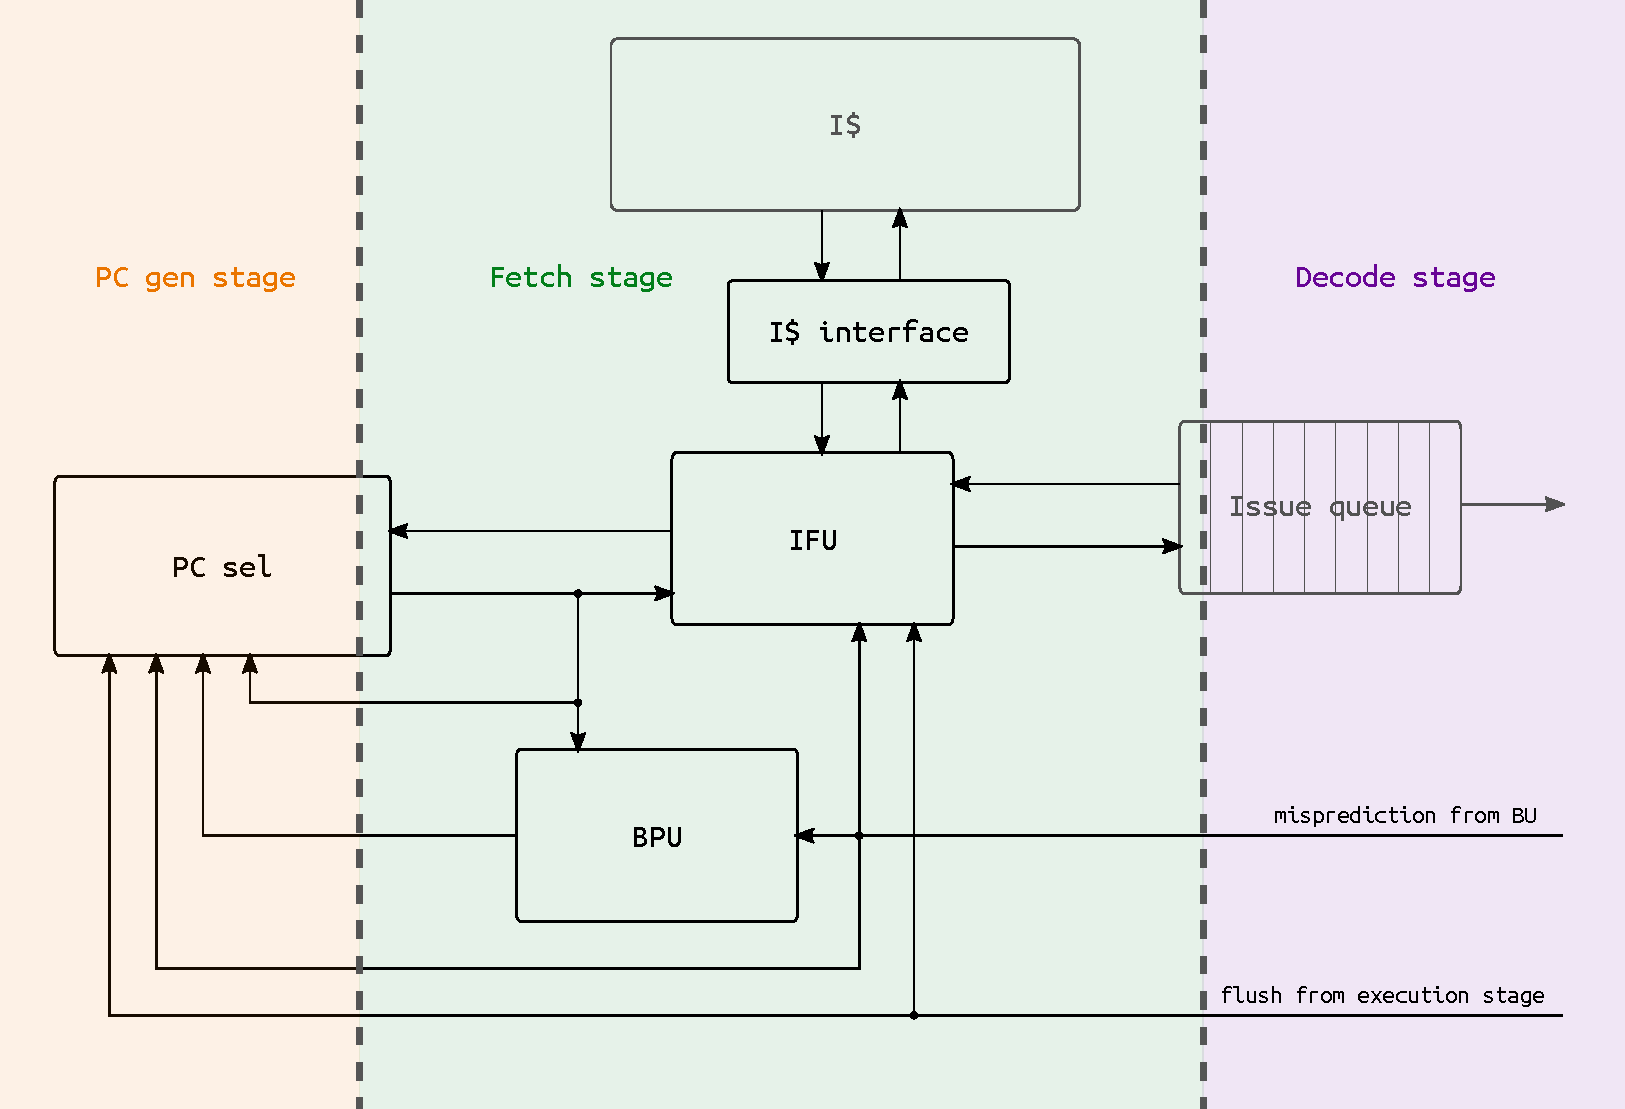
\includegraphics[width=\textwidth]{img/frontend.pdf}
  \caption{LEN5 frontend}
  \label{fig:frontend}
\end{figure}
\Cref{fig:frontend} shows a top-level block diagram of the LEN5 frontend, with the modules that were developed and that will be described in the following sections shown in solid black color. Gray blocks are instead the ones the frontend interfaces with, that are the instruction cache, or equivalently the memory management unit, and the issue queue.

The frontend is composed of two pipeline stages, namely the \emph{\ac{PC} generation} and the \emph{fetch} stages. \Cref{fig:frontend} also shows the \emph{decode} stage, where the issue queue is found. The latter is basically a \acs{FIFO} that serves as a buffer interface between the frontend and the backend of the processor by storing a queue of instructions to be issued to the later stages of the pipeline.

\subsection{\acs{PC} gen stage}
In the \ac{PC} generation (\ac{PC} gen) stage, the next \ac{PC} is selected among a number of different options by the \ac{PC} sel block, using a predefined priority, and is then written on the output register of the stage. This register also serves as the pipeline register between the two stages, and that is why \cref{fig:frontend} shows a dashed gray line crossing the \ac{PC} sel block. 

The selection of the new \ac{PC} is carried out by a network of combinational logic, so that this stage always takes exactly one clock cycle.

\subsection{Fetch stage}
In the fetch stage, the \ac{PC} is used by the \acf{IFU} to select and possibly read from memory the next instruction to be pushed to the issue queue. At the same time, the \acf{BPU} uses the current address to predict the next direction in case of branch and passes such information back to the \ac{PC} gen stage. Memory accesses are performed through the instruction cache interface which manages the control signals to the instruction cache. 

The latency of this stage is at least two clock cycles (see \cref{sec:ifu}); in a normal steady state the \ac{IFU} can provide a throughput of one instruction each clock cycle to the issue queue, but in case of cache miss the number of cycles to resolve the stall can grow significantly, so the latency cannot be determined in advance. The issue queue is there exactly to provide some elasticity to the pipeline, by buffering already fetched instructions, masking at least in part this unpredictable latency.

\subsection{Handshake signals}\label{sec:handshake}
The communication between each stage is always bidirectional, because in case of a stall, caused for instance by a cache miss, by a full issue queue or by some other exceptional behavior down the pipeline, the \ac{PC} generation process must be interrupted along with the fetch. In order to do so, a handshake process handles the communication between each stage as well as between the instruction cache interface and the actual cache.

This handshake mechanism is based on the AXI valid/ready protocol described below, even if it is not compliant with all the AXI specifications.

In each communication the source of data generates a \emph{valid} signal to indicate that the information is available, while the destination generates a \emph{ready} signal to indicate that it can accept such information \cite[p.~A3-41]{axi}. The handshake takes place and the information is successfully exchanged only at the rising clock edge when both valid and ready are asserted. For example, in \cref{fig:axi}, the handshake happens at the third rising edge of the clock.
\begin{figure}[hbt]
  \centering
  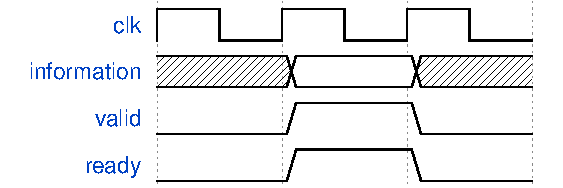
\includegraphics[scale=.9]{img/axi.pdf}
  \caption{AXI handshake protocol}
  \label{fig:axi}
\end{figure}

When a source has information available (\cref{fig:axi_valid_ready}), it must assert valid and then wait until the corresponding ready is produced. It cannot wait for the ready before asserting valid.
\begin{figure}[hbt]
  \centering
  \subfloat[Valid before ready]{
    \label{fig:axi_valid_ready}
    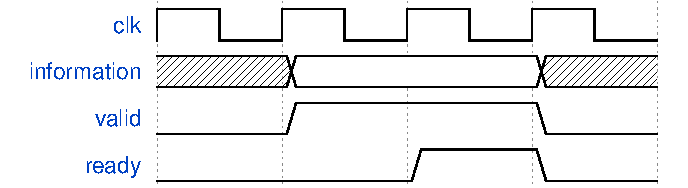
\includegraphics{img/axi_valid_ready.pdf}} \\
  \subfloat[Ready before valid]{
    \label{fig:axi_ready_valid}
    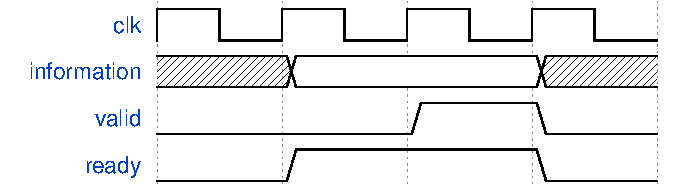
\includegraphics{img/axi_ready_valid.pdf}}
  \caption{Possible handshake timings}
  \label{fig:axi_timings}
\end{figure}
On the other hand (\cref{fig:axi_ready_valid}), a destination is allowed to wait for its valid before asserting ready and it can also deassert ready before a corresponding valid arrives, which is necessary if the destination becomes busy for other reasons.

\section{\acs{PC} gen stage}
The selection of the next \ac{PC} is based on the following list of priorities, from highest to lowest:
\begin{enumerate}
  \item \textbf{Exception}\footnote{Or interrupt. The two terms can be used almost interchangeably in \riscv.}: if an exception occurs, the \ac{PC} gen stage will receive the next starting address as the base address present in the vector table provided by the CSR unit.
  \item \textbf{Misprediction}: if a resolved branch is discovered to have been mispredicted, then the \ac{PC} gen stage resumes execution from the correct target if the branch was actually taken, or from the next sequential address from the branch \ac{PC} if it was actually not taken.
  \item \textbf{Branch prediction}: if the \ac{BPU} predicts a taken branch for the current \ac{PC} then it provides this stage with the predicted target address (see \cref{sec:btb}), which will be fetched at the next cycle, thus allowing for zero penalty branches when predicted correctly.
  \item \textbf{Default assignment}: if none of the conditions before occur, then the next \ac{PC} is selected as usual as the next sequential address, which corresponds to the current \ac{PC}+4 for word-aligned 32-bit instructions.
\end{enumerate}

\begin{figure}[hbt]
  \centering
  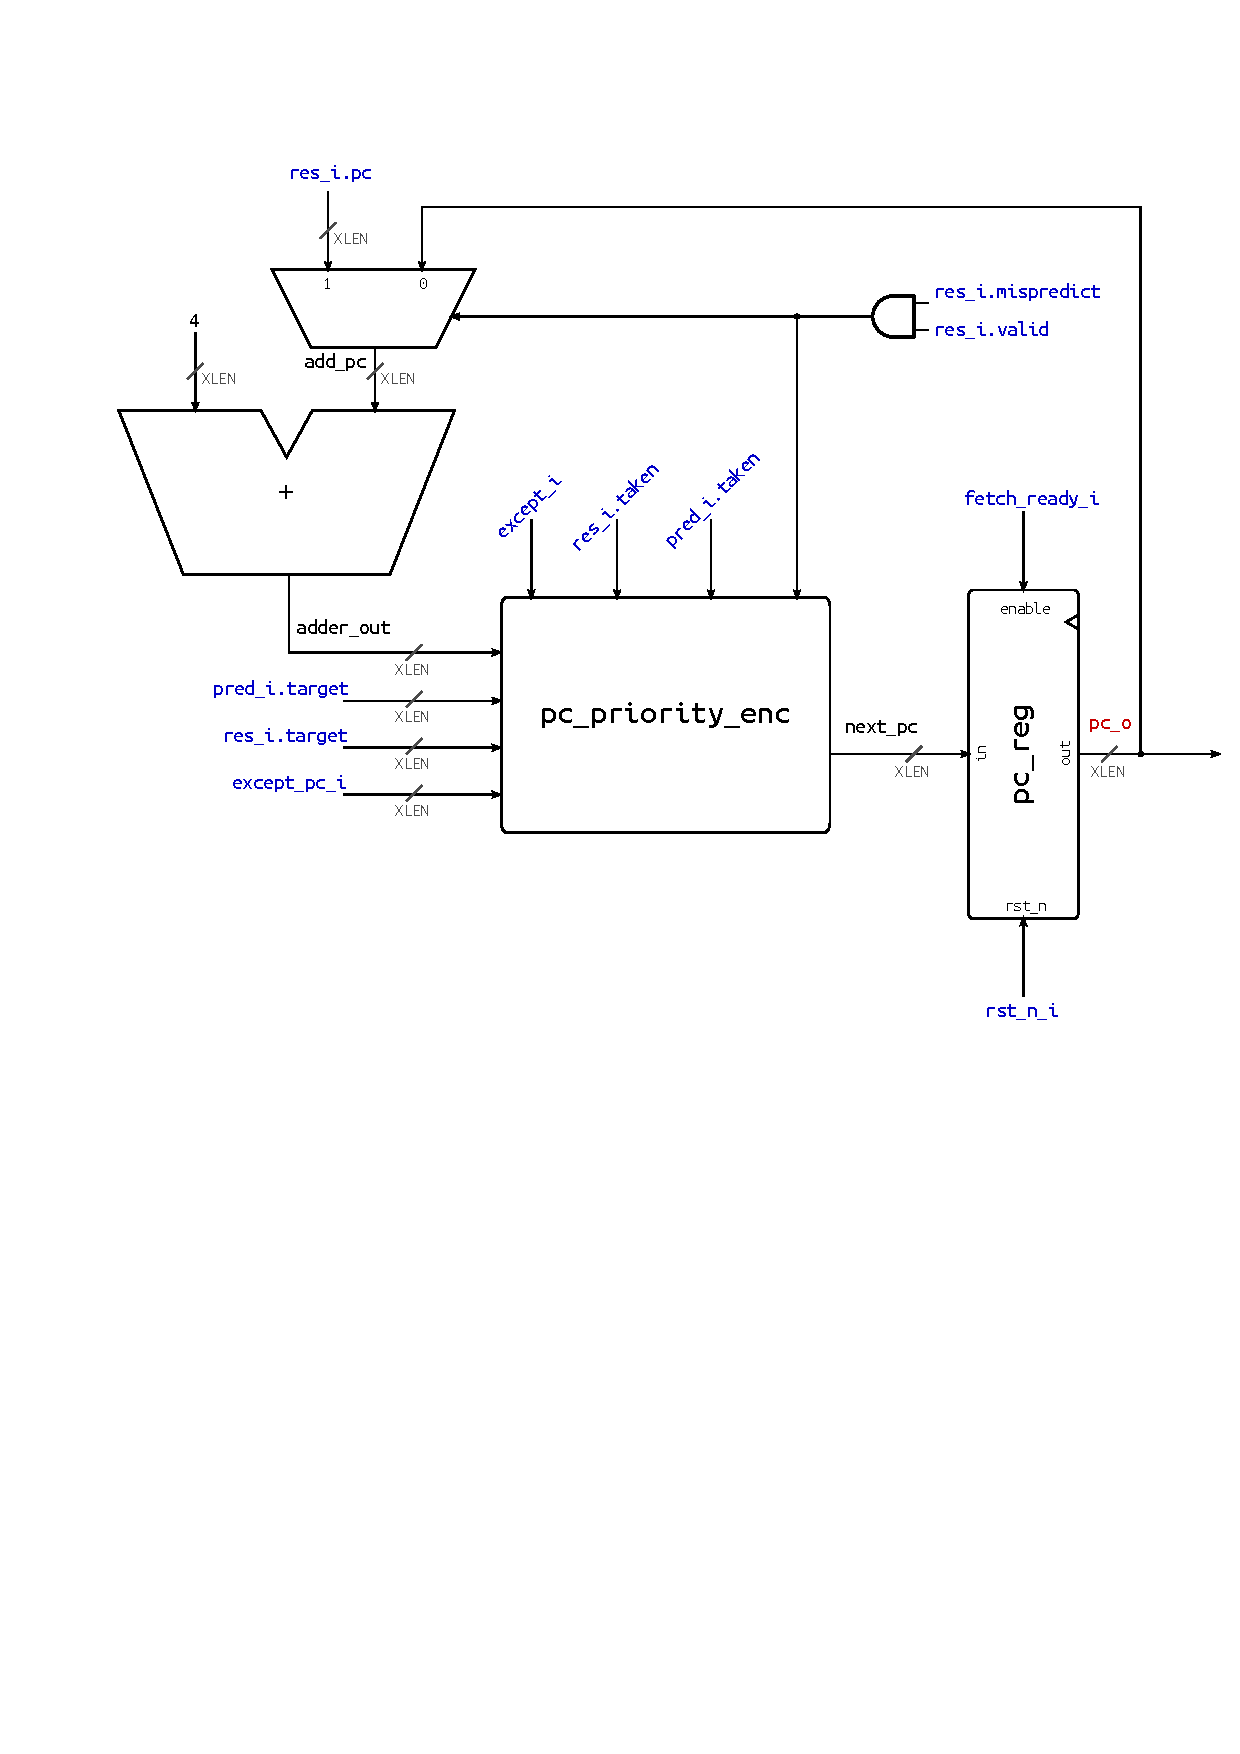
\includegraphics[width=\textwidth]{img/pc_gen_stage.pdf}
  \caption{\acs{PC} gen stage diagram}
  \label{fig:pc_gen_stage}
\end{figure}
\Cref{fig:pc_gen_stage} shows the diagram of this stage. This and all the following diagrams in this document are color coded so that input signals are in {\color{input_blue}{blue}} and have the suffix \texttt{\_i}, output signals are in {\color{output_red}{red}} and have the suffix \texttt{\_o}, internal signals in black and bit widths are in {\color{width_gray}{gray}}.

The heart of the \ac{PC} gen stage is the \texttt{pc\_priority\_enc} block, which is an encoder that takes as inputs all the status signals indicating a behavior different from the default and all the corresponding potential next \acp{PC}. In behavioral SystemVerilog (\cref{code:priorityenc}) it is described as an if-then-else chain, which gets synthesized as a list of cascading multiplexers implementing the desired priority\footnote{As opposed to the description using a case statement, which leads to a single parallel mux, with no priority encoded.}.

\begin{minipage}{\textwidth}
  \begin{lstlisting}[
    language=Verilog,
    caption={\texttt{pc\_priority\_enc} description},
    captionpos=b,
    label=code:priorityenc
  ]
    always_comb begin: pc_priority_enc
      if (except_i) begin
        next_pc = except_pc_i;
      end else if (res_i.valid && res_i.mispredict) begin
        if (res_i.taken) begin
          next_pc = res_i.target;
        end else begin
          next_pc = adder_out;
        end
      end else if (pred_i.taken) begin
        next_pc = pred_i.target;
      end else begin
        next_pc = adder_out;
      end
    end: pc_priority_enc
  \end{lstlisting}
\end{minipage}

In order to save resources, a single adder is used to generate both the next sequential address and the next \ac{PC} after a mispredicted not taken branch. A multiplexer driven by the misprediction signals is used to select the right operand.

The final chosen next \ac{PC} is fed into the \texttt{pc\_reg} output register for the later stages. The enable of this register is controlled by the signal \texttt{fetch\_ready} which comes from the fetch stage and disables the \ac{PC} generation if a stall occurs. This is part of the handshake mechanism described in \cref{sec:handshake}, even if there is no \emph{valid} signal from the \ac{PC} gen stage, as it is redundant due to the fact that a valid new \ac{PC} is always present at the output register.

\section{Instruction cache interface}
\todo{Talk about FSM coding style}
\begin{figure}[hbt]
  \centering
  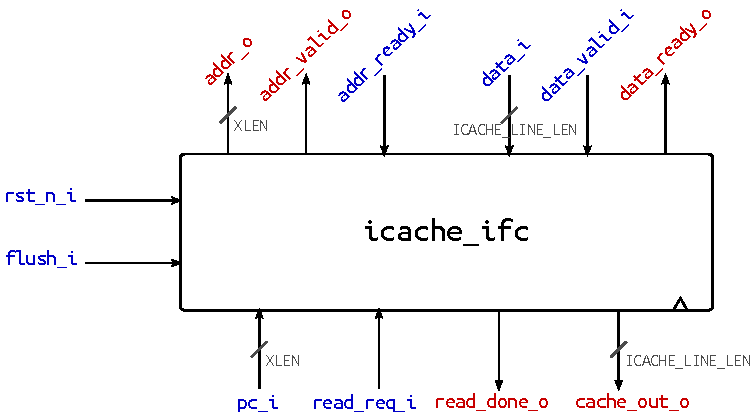
\includegraphics{img/icache_ifc-top.pdf}
  \caption{Instruction cache interface module ports}
  \label{fig:icache_ifc-top}
\end{figure}
The instruction cache interface (\cref{fig:icache_ifc-top}) is responsible for translating the fetch requests coming from the \ac{IFU} into compliant valid/ready handshake signals for both address and data to the instruction cache. This unit basically provides two main benefits. First, it simplifies the control of the \ac{IFU}, by delegating the handshake process. Second, and more important, it provides an additional separation layer between the core frontend and the instruction cache with modularity in mind so that, should the cache block be modified, only this interface unit needs to be updated, while the signals coming from the \ac{IFU} module would remain unchanged.

\subsection{Datapath}
\begin{figure}[hbt]
  \centering
  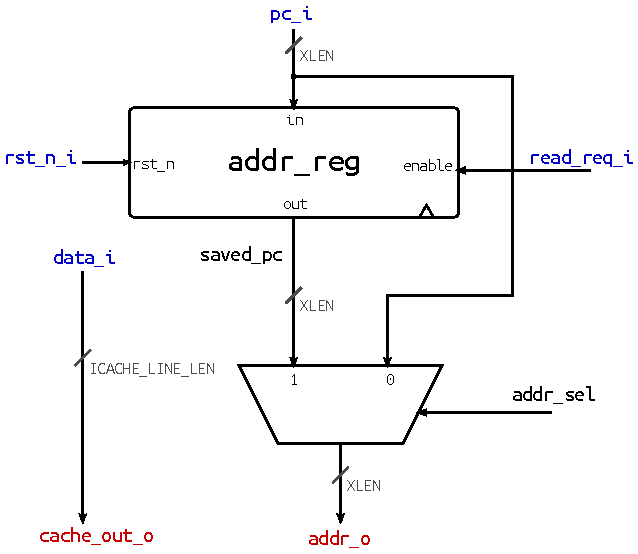
\includegraphics{img/icache_ifc.pdf}
  \caption{Instruction cache interface datapath}
  \label{fig:icache_ifc}
\end{figure}
For what concerns data signals, the line received from the instruction cache is directly connected with the \texttt{cache\_out} output, as it is the cache itself that is responsible for keeping its output valid until the handshake occurs. On the other hand, no assumption can be done on the timing of the input address other than the fact that it will be valid in the same cycle when \texttt{read\_req} is asserted. For this reason, given the possibility for the \ac{PC} to change at the following cycle, the requested address must be retained inside the interface by means of a register, as shown in \cref{fig:icache_ifc}. The multiplexer selects the input address if the cache is ready to receive the address in the cycle the request is sent, otherwise it selects the registered address in the following cycles.

\subsection{Control \acs{FSM} and timing}
\begin{figure}[hbt]
  \centering
  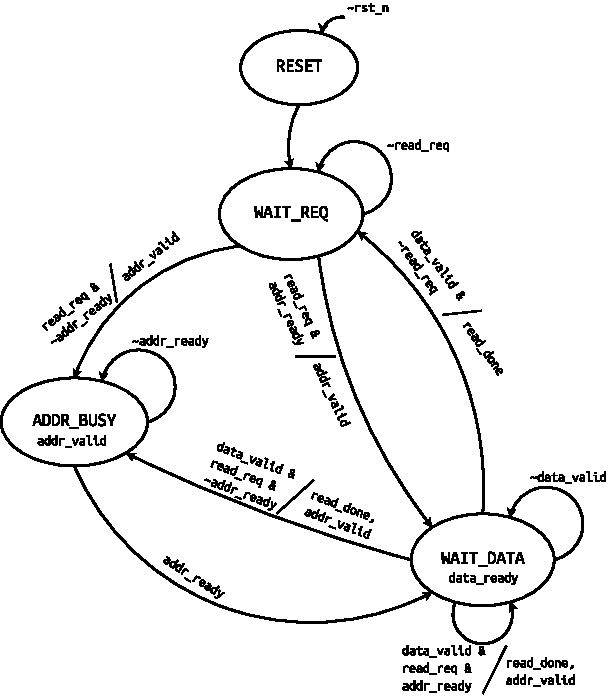
\includegraphics[scale=1]{img/icache_ifc_fsm.pdf}
  \caption{Instruction cache interface \acs{FSM}}
  \label{fig:icache_ifc_fsm}
\end{figure}
The control unit of this block is a simple Mealy \acs{FSM} (\cref{fig:icache_ifc_fsm}) that after reset waits for a read request from the \ac{IFU}, then checks if the instruction cache is ready to receive an address and finally waits for a valid cache line to be read.

Read requests can be accepted both in the idle \texttt{WAIT\_REQ} state and in the \texttt{WAIT\_DATA} state, in order to ensure maximum throughput by initiating the next memory access in the same clock cycle as the data handshake of the previous one.

\begin{figure}[hbt]
  \centering
  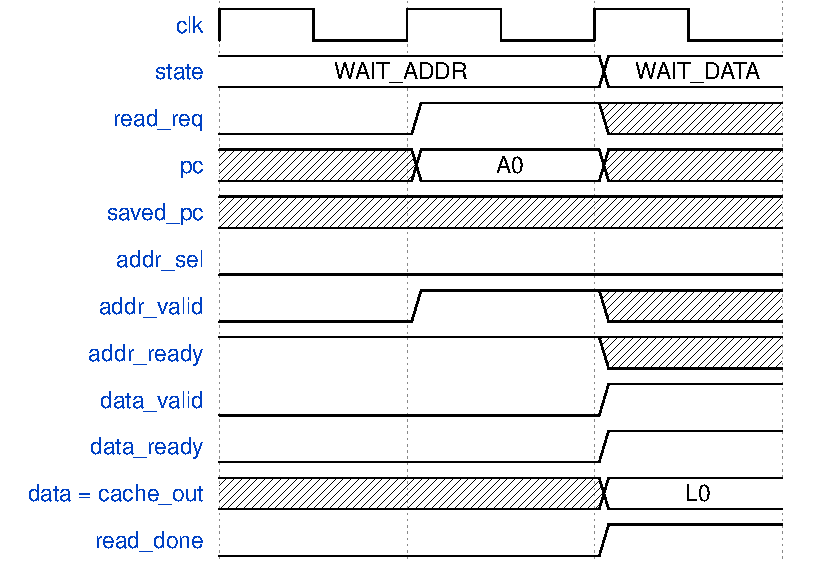
\includegraphics{img/cache01.pdf}
  \caption{Normal cache read}
  \label{fig:cache01}
\end{figure}
\Cref{fig:cache01} shows a normal cache read, where the instruction cache is immediately ready to receive an address which hits and produces the requested data at the next clock cycle. From this timing diagram it is also clear why a Mealy \acs{FSM} is needed: the signal \texttt{addr\_valid} needs to be asserted combinationally in the same clock cycle in which \texttt{read\_req} arrives, so that the address handshake can take place immediately. Otherwise, with a Moore machine, one clock cycle would be wasted at each request, rendering impossible to sustain one instruction per clock cycle fetch. Another possibility would have been not to include such signal as a Mealy output of the machine and instead connect it with a wire outside the \acs{FSM}, which would lead to the same exact result, but was deemed as less readable.

\begin{figure}[hbt]
  \centering
  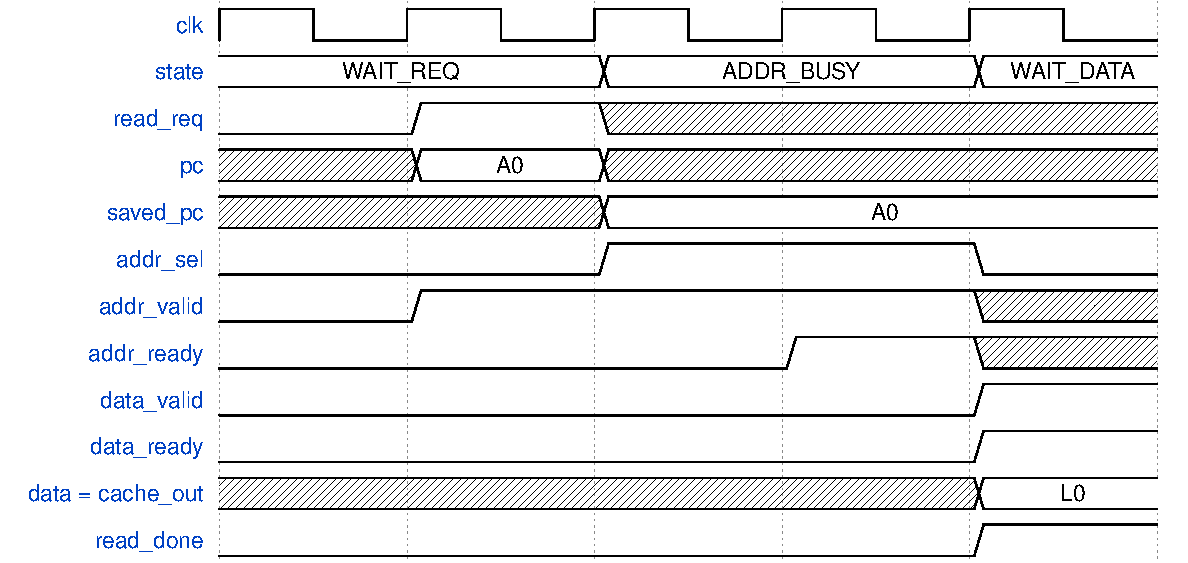
\includegraphics[width=\textwidth]{img/cache02.pdf}
  \caption{Cache not ready on address}
  \label{fig:cache02}
\end{figure}
\Cref{fig:cache02} shows another possibility when the instruction cache is not ready to receive an address at the time when a request arrives. In this case the \acs{FSM} waits until the cache become ready in the \texttt{ADDR\_BUSY} state. The state machine could just as well wait in the \texttt{WAIT\_REQ} state, but the additional state was introduced for robustness with \texttt{addr\_valid} as a Moore output, so that this way there is no need for the \texttt{read\_req} signal to stay active until the cache is ready. This is another point in favor of a Mealy \acs{FSM} instead of the connection of combinational outputs externally. Moreover, if the \acs{FSM} loops in this waiting state, the registered address is selected for the handshake, as the original program counter could have changed by that point. 

\begin{figure}[hbt]
  \centering
  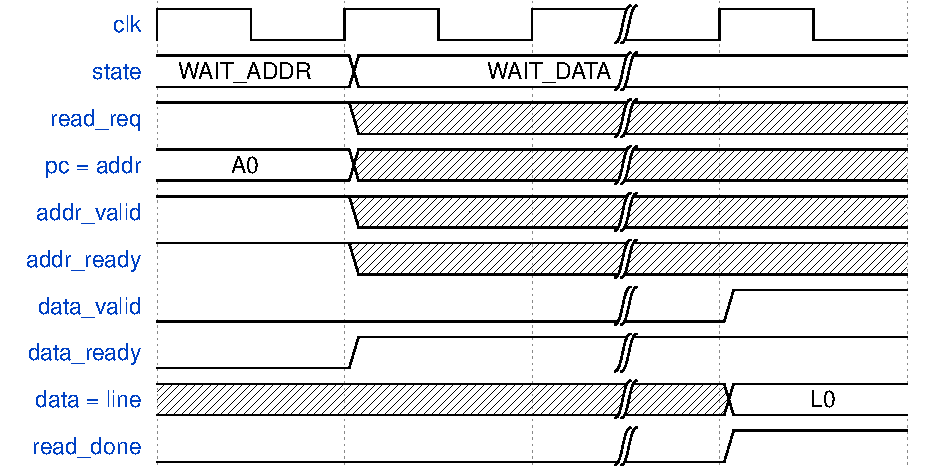
\includegraphics[width=\textwidth]{img/cache03.pdf}
  \caption{Cache miss}
  \label{fig:cache03}
\end{figure}
Finally, \cref{fig:cache03} shows the case of a cache miss, in which the \acs{FSM} waits while keeping \texttt{data\_ready} asserted. This state could potentially last for many clock cycles.

\section{\acf{IFU}}\label{sec:ifu}
\begin{figure}[hbt]
  \centering
  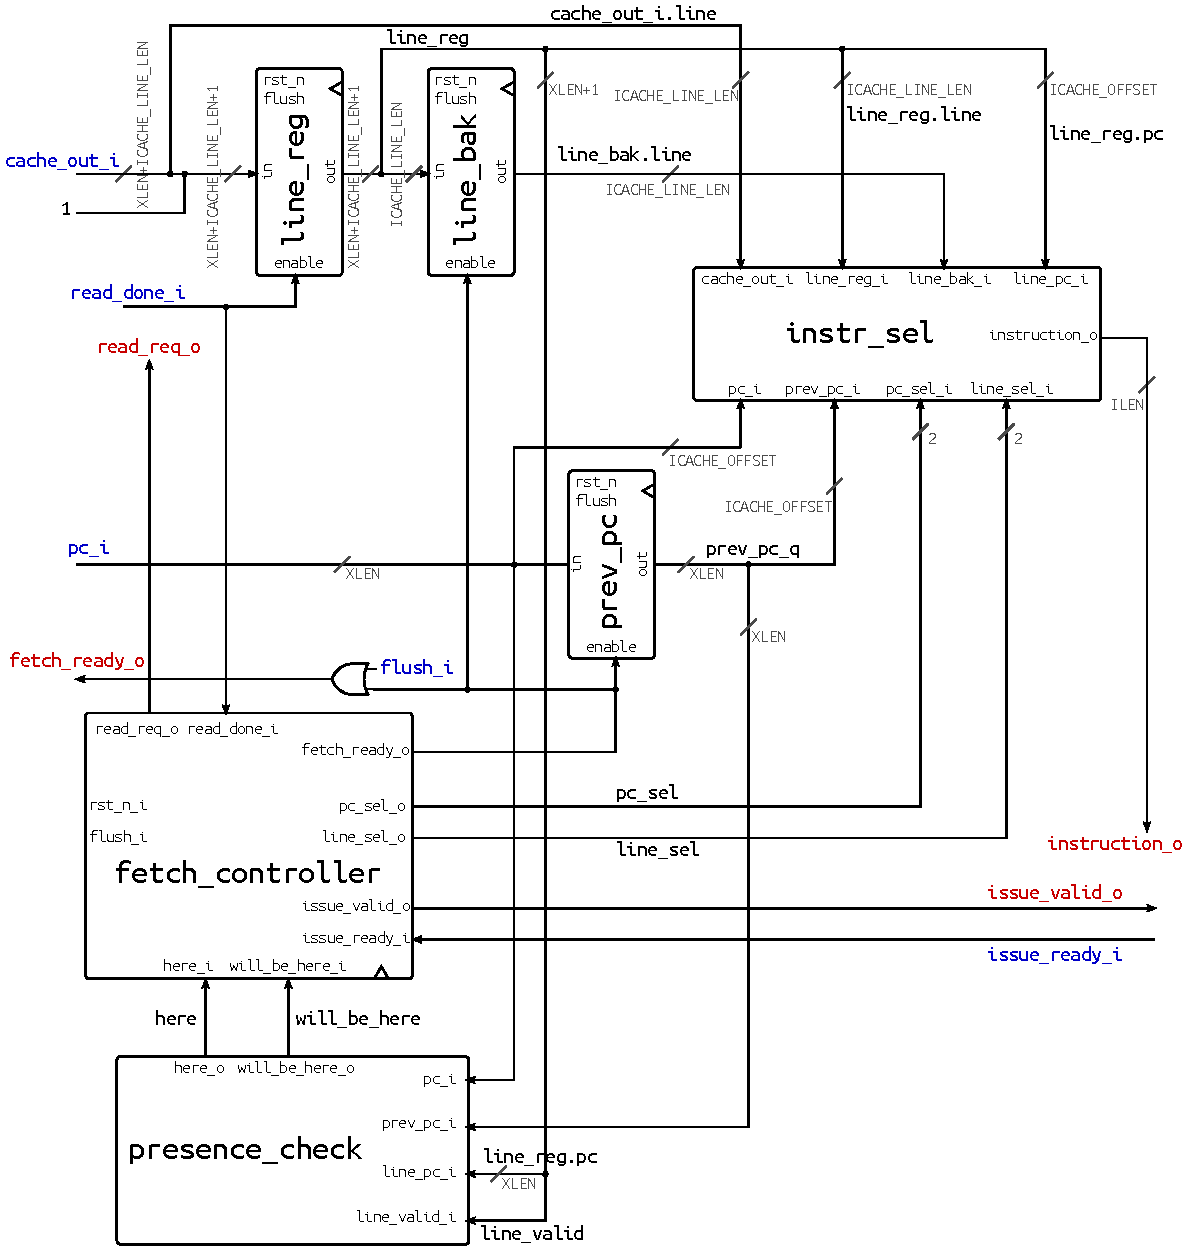
\includegraphics[width=\textwidth]{img/ifu.pdf}
  \caption[\acs{IFU} diagram]{\acs{IFU} diagram (inputs \texttt{rst\_n\_i} and \texttt{flush\_i} are shown as module port but are not connected with wires to avoid further clutter in the diagram, apart from the output OR gate)}
  \label{fig:ifu}
\end{figure}
\Cref{fig:ifu} shows the top level diagram of the \ac{IFU}, which has the ability to fetch instructions from thee different locations. The first is the direct output of the instruction cache, from which instructions are taken in case of a memory access. Then, when a cache line containing multiple instructions is read, it is saved into a \emph{line register} along with a valid bit that indicates that such line is valid. Consecutive instructions belonging to the same cache line are then fetched from this register, thus reducing the total number of cache requests. Finally, this line register is in turn saved into a \emph{line backup register} every time that a fetch takes place (i.e.\ the register is not updated during a stall). This additional location is used every time that the current \ac{PC} requires a cache access, but the next address refers to an instruction that was present in the previously saved cache line. Without a backup, the line register would be overwritten by the line fetched at the current \ac{PC} and so the next address would require a new cache read. Using an additional register, on the other hand, allows the \ac{IFU} to read the next instruction from the previous line. Evidently, this reasoning could be iterated to account for the second-oldest, third-oldest, etc. saved cache line, leading to a longer \acs{FIFO} of line registers among which to select the current instruction. This is definitely a possible improvement, but including more than two registers was judged out of the scope of the frontend. An actual improvement should on the other hand come from the memory system, that could for instance include a \emph{trace cache}, to account for subsequent instructions frequently fetched from different cache lines. Should such a feature be included, no other modifications would be needed on the \ac{IFU} end.

Two blocks, namely the \emph{presence checker} and the \emph{instruction selector} are responsible of informing the fetch controller if the current \ac{PC} points to an instruction already present in a saved line and of choosing the right source and the right instruction in the cache line respectively. The fetch controller itself is responsible of the orchestration of all the operations carried out inside the \ac{IFU} and of interfacing with the instruction cache interface as well as the \ac{PC} gen stage before and the issue queue after.

At the startup of the processor, the first fetch address will be the defined boot address which it is safe to assume that is going to need a cache access, as no line has been read and saved yet in the line register. This means that, even in the best case scenario (i.e.\ cache hit), the first instruction will be pushed to the issue queue one clock cycle after the corresponding \ac{PC} has entered the fetch stage, leading to a latency of a total of two clock cycles. In order to maintain the throughput of one instruction per clock, however, the \ac{PC} generation process must go on before knowing if the cache will hit or miss and that means that the first \ac{PC} must be saved in a \emph{previous \ac{PC} register} in order to push the correct instruction to the queue at the next cycle. In other words, at each clock cycle, the \ac{IFU} is simultaneously checking whether the current \ac{PC} refers to a saved instruction or if a cache access is needed and pushing the previous instruction to the issue queue. Actually, if the current instruction is already present in a line register, then it could be potentially moved to the queue in the same cycle as no cache latency must be accounted for. This, however, would complicate significantly the timing of this unit, as the latency would be variable according to the need of a cache read or otherwise. For this reason, it has been chosen to maintain a one-cycle latency for every instruction, meaning that each instruction pushed to the queue corresponds to the \ac{PC} of the previous cycle. This is effectively an additional pipeline stage, introduced to account for the minimum cache latency and not to reduce the critical path.

Finally, in case of an exceptional behavior or a branch misprediction, the \ac{IFU} must be flushed and all pending cache requests aborted, in order to resume the process at the next cycle when the new starting \ac{PC} will be provided by the \ac{PC} gen stage. In order to do so, a \texttt{flush} signal that comes from the later execution stages or from the top-level control is propagated to all the sequential elements of the \ac{IFU}. This acts as a synchronous reset for all the registers and reverts back all the \acsp{FSM} to their startup state \cite{resets}, by acting directly on the state register. For this latter case, the effect is the same of having a check on the flush signal in each state of the machine, but leaving it as an external signal similar to the initial reset simplifies significantly the state diagram and helps readability.

\subsection{Presence checker}
\begin{figure}[hbt]
  \centering
  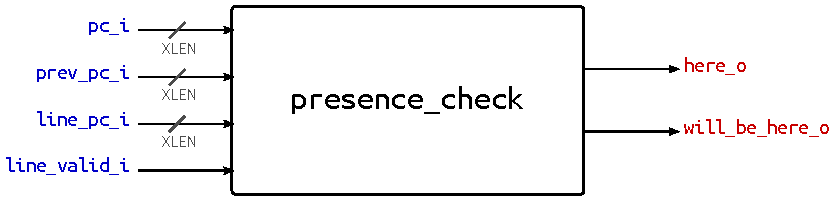
\includegraphics{img/presence_check-top.pdf}
  \caption{Presence checker module ports}
  \label{fig:presence_check-top}
\end{figure}
\begin{figure}[hbt]
  \centering
  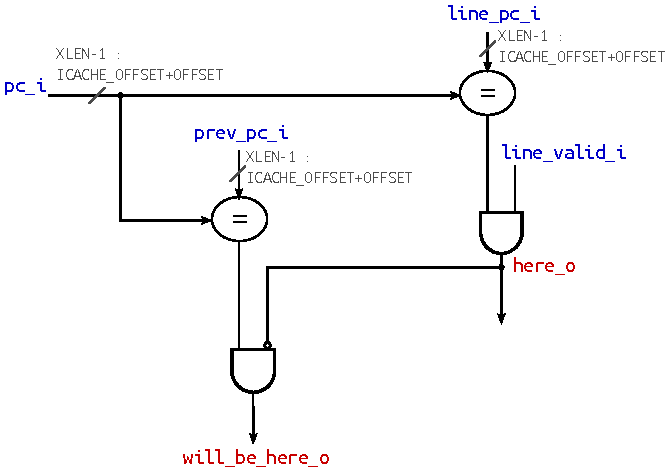
\includegraphics{img/presence_check.pdf}
  \caption{Presence checker combinational network}
  \label{fig:presence_check}
\end{figure}
The presence checker block (see \cref{fig:presence_check-top,fig:presence_check}) features a simple combinational network that performs two checks in parallel to determine the need of a new cache access by the \ac{IFU}, in particular:
\begin{itemize}
  \item If the current address refers to an instruction present in the line register and the saved line is valid, then the \texttt{here} signal indicates that no new cache read is needed and that the instruction is to be selected inside the line register.
  \item If the current address refers to an instruction in the same cache line as the previous address, then either that line is already present in the line register, or it will be the next line read from the cache and so it will be saved as soon as the read completes. In this case a \texttt{will\_be\_here} signal tells the \ac{IFU} not to request the same line twice to the memory. 
\end{itemize}
If none of these signals are asserted, then a new cache request is sent to the interface.

All the instructions belonging to the same cache line have the same most significant parts of the address, that is, only the $N$ LSBs differ, where:
\begin{equation*}
  N = \lceil \log_2(\text{Instructions/cache line}) \rceil + 
      \lceil \log_2(\text{Bytes/instruction}) \rceil
\end{equation*}
So, to check whether two instructions belong to the same line, a comparison between the $64-N$ (or more generally $\texttt{XLEN}-N$, where \texttt{XLEN} is the parallelism of the processor) most significant bits of their addresses is sufficient. That is what the presence checker does as shown in \cref{fig:presence_check}.

\subsection{Instruction selector}
\begin{figure}[hbt]
  \centering
  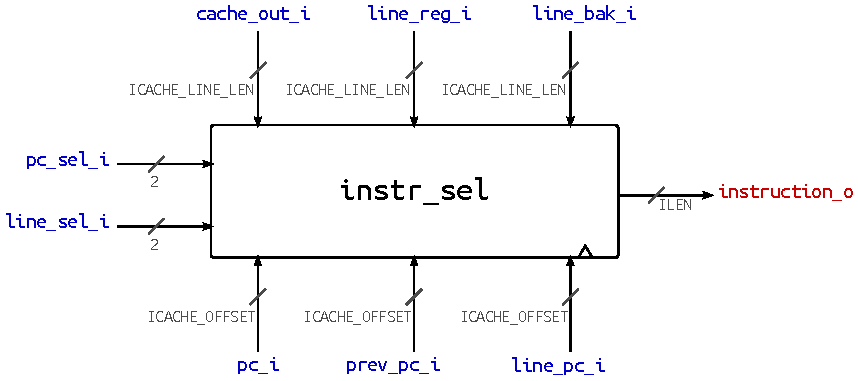
\includegraphics{img/instr_sel-top.pdf}
  \caption{Instruction selector module ports}
  \label{fig:instr_sel-top}
\end{figure}
\begin{figure}[hbt]
  %\hspace*{-1.5cm}
  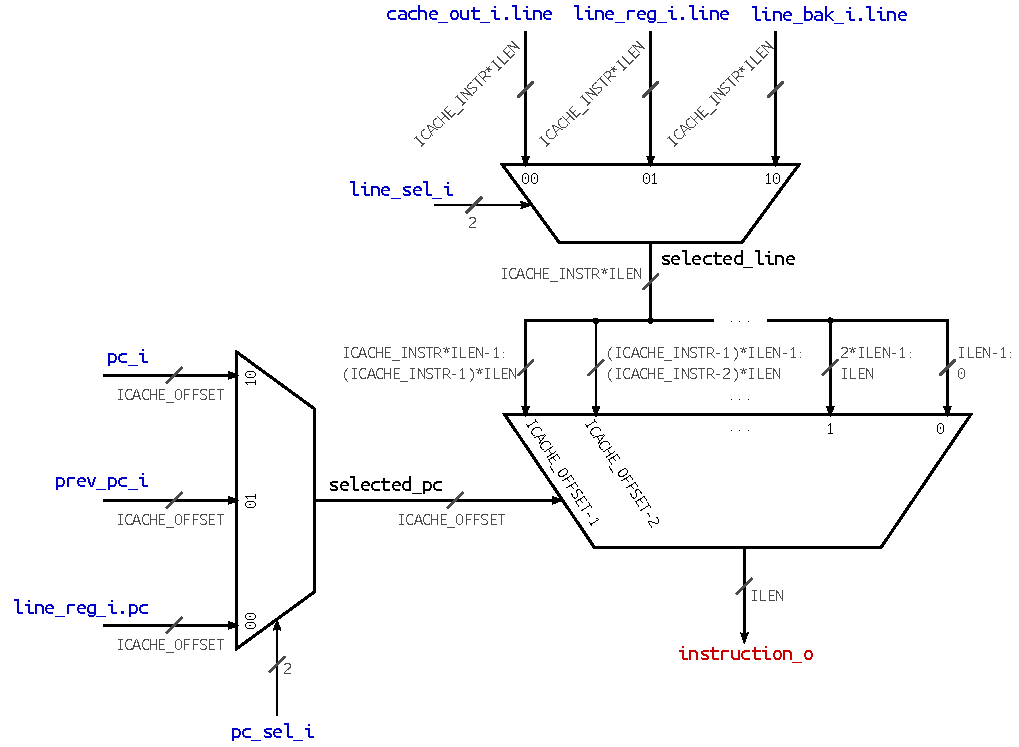
\includegraphics[width=\textwidth]{img/instr_sel.pdf}
  \caption{Selection network}
  \label{fig:instr_sel}
\end{figure}
The instruction selector takes as inputs all the three sources an instruction can be fetched from, three program counter sources\footnote{The only source actually used, as stated above, is the previous \ac{PC}, but the others were included in the initial version of the design and have been kept should a future need arise. Given that the synthesizer can optimize unused wires, this choice incurs no overhead.} and the respective selection signals (see \cref{fig:instr_sel-top}). It outputs a single selected instruction to be pushed to the issue queue.

\Cref{fig:instr_sel} shows the combinational selection network of the instruction selector, which basically consists of two multiplexers selecting the desired cache line and the address pointing to that line and another multiplexer choosing the selected instruction inside such line.

According to the number of instructions stored in a single cache line, the output multiplexed can become quite large, nonetheless it should not be an issue in terms of total area.

\subsection{Fetch controller}
\begin{figure}[hbt]
  \centering
  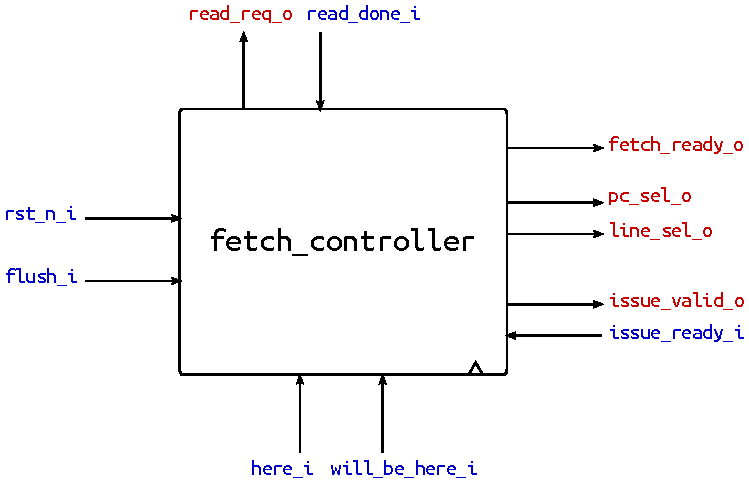
\includegraphics{img/fetch_controller-top.pdf}
  \caption{Fetch controller module ports}
  \label{fig:fetch_controller-top}
\end{figure}
The fetch controller module, whose interface is shown in \cref{fig:fetch_controller-top}, is the control unit of the \ac{IFU} which is responsible of receiving and generating control signals both for internal blocks and for interfacing with the other stages and the instruction cache. In particular, the controller receives information about saved instructions by the presence checker block (\texttt{here} and \texttt{will\_be\_here} signals) and as a consequence determines if a cache access is needed (\texttt{read\_req} and \texttt{read\_done} interface signals) and drives the correct selection signals (\texttt{pc\_sel} and \texttt{line\_sel}) to the instruction selector block.

Moreover, it handles the handshake signals \texttt{issue\_valid} and \texttt{issue\_ready} to and from the issue queue. The valid is asserted every time that the fetched instruction is available, as the result of a cache hit or saved in the line registers, while the ready signals that the issue queue is not full and has at least available room for one more instruction. 

Finally, the \texttt{fetch\_ready} signal is used in the \ac{PC} gen stage as the enable of the output register (see \cref{fig:pc_gen_stage}) and in the fetch stage as the enable of the previous \ac{PC} register (see \cref{fig:ifu}). This signal is deasserted in the case of a stall, that in particular can occur if the cache misses on the requested address or if the issue queue is full and cannot accept more instructions. Note that in case of flush, however, this signal remains active, because the flush operation resets all the data structures in one clock cycle and at the next the \ac{IFU} is again ready to fetch, so the \ac{PC} gen stage must provide the new valid start address.

\subsubsection{Control unit}
The main difficulties reside in high number of possible combinations of events that can occur simultaneously. For instance the issue queue could become full while a memory access is being completed, or on the other hand while an instruction is being selected in the line register. These different conditions must be handled in a per-case manner and that is what the Mealy machine of \cref{fig:fetch_controller_fsm} manages. Here follows a summary of the purpose of each state:
\begin{figure}[hbt]
  \centering
  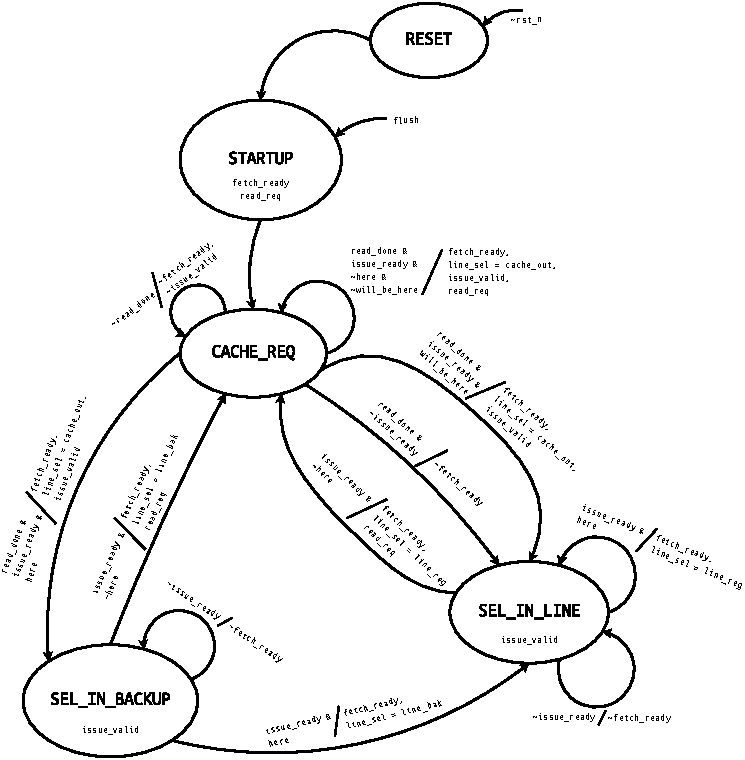
\includegraphics[width=\textwidth]{img/fetch_controller_fsm.pdf}
  \caption{Fetch controller \acs{FSM}}
  \label{fig:fetch_controller_fsm}
\end{figure}
\begin{itemize}
  \item \texttt{STARTUP}: this state can occur only after a reset or a flush. In both cases, at that moment the \ac{PC} corresponds to the starting address and all the line registers have been reset to zero, so a new cache read is necessary and the \texttt{read\_req} signal is asserted as a Moore output. The reason why the \ac{PC} is already valid and correct at this cycle is due to the fact that, in case of reset, the output register of the \ac{PC} gen stage is not reset to zero, but to the a constant \texttt{BOOT\_ADDRESS} that initiates the program execution. In case of flush, on the other hand, the \ac{PC} is set to the next address in the following cycle with respect to when the flush signal arrives, thanks to the OR gate (see \cref{fig:ifu}) that enables the \ac{PC} register in case of flush, even if the \texttt{fetch\_ready} signal would have prevented it. The latter is the other Moore output in this state and is needed, as stated before, to ensure maximum throughput before knowing if the cache will have a hit or miss (i.e.\ the next \ac{PC} is generated nonetheless and in case of miss the \ac{IFU} is stalled at the following cycle).
  \item \texttt{CACHE\_REQ}: in this state a memory access request is sent to the instruction cache interface. In case the cache is not ready to receive the address or incurs a miss, then the \acs{FSM} loops in this state until the \texttt{read\_done} signals is asserted, stalling the frontend by deasserting \texttt{fetch\_ready}. 
  
  When the miss is resolved or immediately in case of hit, the state machine checks if the issue queue is ready. If it is, then the instruction is pushed and according to the output of the presence checker in that cycle, the next state transition is determined. If \texttt{here} is asserted, it means that the next instruction is present in the previously saved cache line, so at the next cycle, when the cache line just read will be saved in the line register and the old line register will be saved into the line backup register, the instruction will be selected from the backup register (move to \texttt{SEL\_IN\_BACKUP} state). If \texttt{will\_be\_here} is asserted, it means that the next instruction belongs to the same line that was just read, so it will be selected from the line register at the next cycle (move to \texttt{SEL\_IN\_LINE} state). If otherwise none of these signals are active, the next instruction belongs to a totally different cache line and so another memory access is necessary and the \acs{FSM} stays in this state.

  If the issue queue is full or busy, on the other hand, the cache output will be saved to the line register at the next cycle nonetheless, but the handshake with the queue does not take place and the state machine transitions to \texttt{SEL\_IN\_LINE} where it loops until the issue queue becomes ready again. During this time, the line register will not be updated anymore as the fetch is stalled and no new memory accesses can be performed. \todo{Solution to mask a potential cache miss here?}
  \item \texttt{SEL\_IN\_LINE}: as mentioned above, in case the issue queue is busy, the \acs{FSM} loops in this state waiting. On the contrary, if the queue is ready, an instruction is pushed and then the state machine remains in this state if \texttt{here} is active, signaling that the next instruction will be selected from the same saved line, or moves to \texttt{CACHE\_REQ} otherwise to initiate a new cache request.
  \item \texttt{SEL\_IN\_BACKUP}: this state is the dual of \texttt{SEL\_IN\_LINE} meaning that the \acs{FSM} loops here when the issue queue is full and goes to \texttt{CACHE\_REQ} if the next instruction is not saved anywhere, but with the difference that, if the \texttt{here} signal is asserted, the next state is \texttt{SEL\_IN\_LINE}, where the instruction will be selected in the line register.
\end{itemize}

For the same reasons stated before, it should be easy to understand how a Moore machine would not suit this particular control unit. As an example, with a Moore machine, from the conclusion of a cache read to the push of the selected instruction to the issue queue one clock cycle is bound to be wasted, which would hinder the throughput of the \ac{IFU}.

\subsubsection{Timing diagrams}\label{sec:frontend_timings}
To better understand the behavior of the fetch controller \acs{FSM}, a list of timing diagrams covering a number of possible scenarios is now presented.

\begin{figure}[hbt]
  \centering
  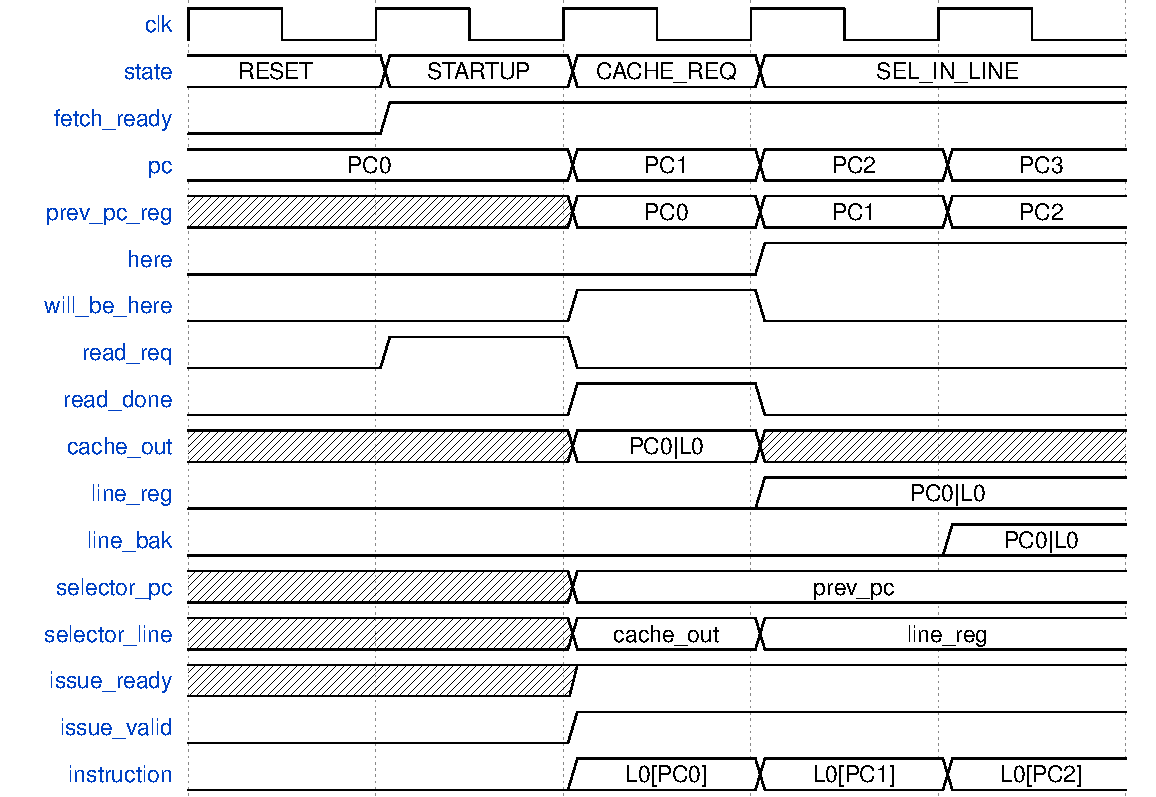
\includegraphics[scale=.6]{img/fetch01.pdf}
  \caption[Startup and hit]{Startup and hit (\texttt{PC0} is the \texttt{BOOT\_PC} considered above)}
  \label{fig:fetch01}
\end{figure}
\Cref{fig:fetch01} shows the boot up after the reset, where the first \ac{PC} needs a cache access and then the next instructions are fetched consecutively from the same line, now saved in the line register. This is the most ideal situation, with a cache hit and the issue queue ready. It is clear from this timing diagram that the \texttt{fetch\_ready} signal must be active during \texttt{STARTUP} even if the outcome of the cache request is not yet known. If this were not the case, there would be a one-cycle penalty every time.

\begin{figure}[!ht]
  \centering
  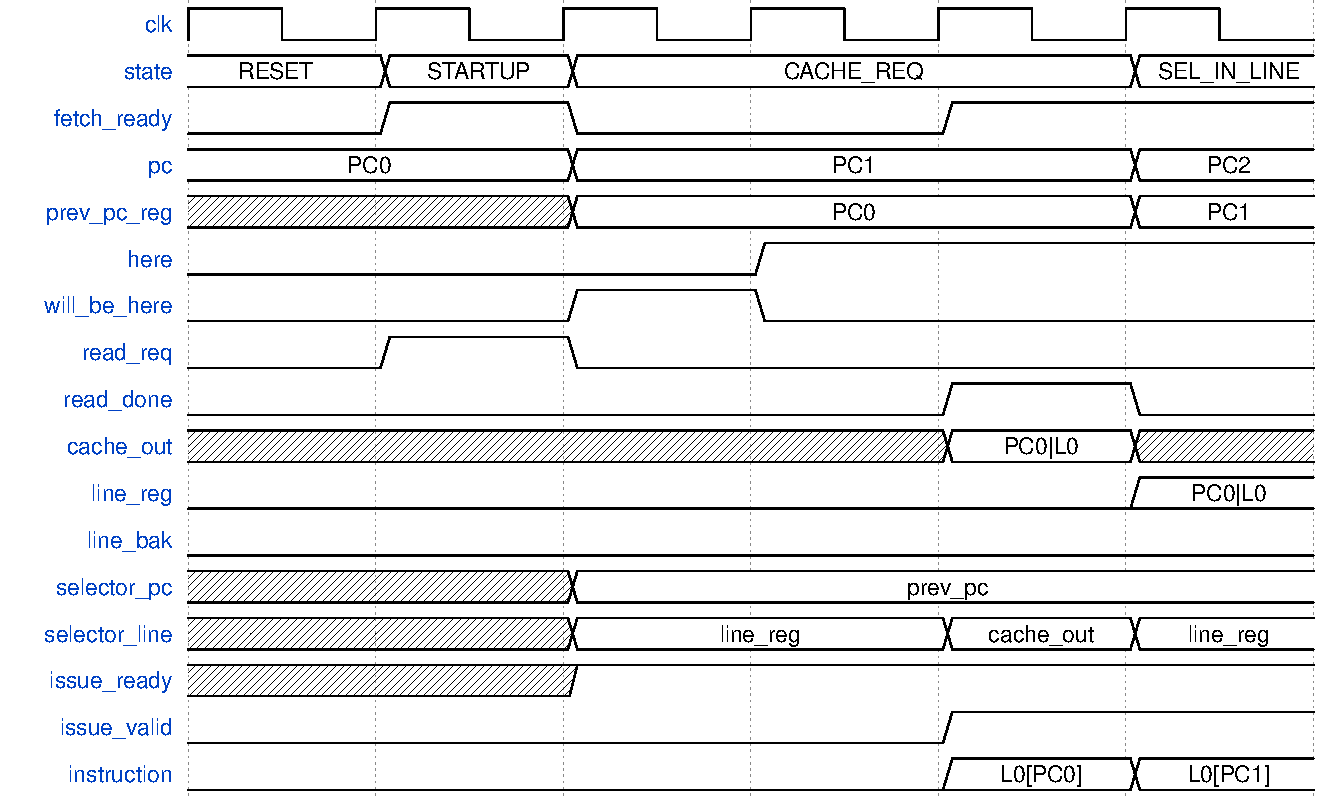
\includegraphics[scale=.6]{img/fetch02.pdf}
  \caption{Startup and cache not ready/miss}
  \label{fig:fetch02}
\end{figure}
\Cref{fig:fetch02} shows what happens in the same situation if instead the cache is not ready or has a miss. This timing also explains why the instruction cache interface must save the address as soon as a read request is sent: if the address handshake does not occur at the second cycle when the request is made, then the address changes at the next clock and the read would happen at the new, wrong address.

\begin{figure}[!hb]
  \centering
  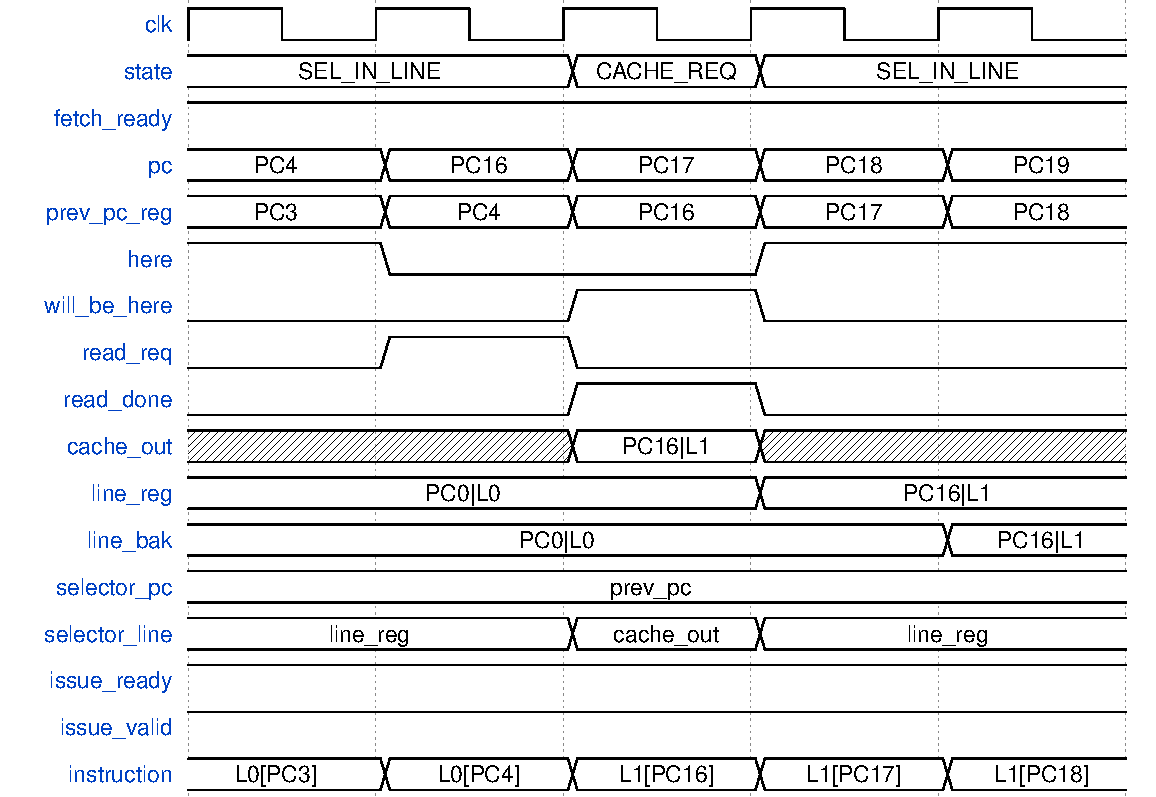
\includegraphics[scale=.7]{img/fetch06.pdf}
  \caption{Saved line change}
  \label{fig:fetch06}
\end{figure}
\Cref{fig:fetch06} shows the situation of a cache line change. At first instructions are read consecutively from the line register, then a branch for example makes the \ac{PC} jump to a location stored on a different cache line, so a read request is sent, the cache hits and the current instruction is read from the cache output. After that, fetch continues sequentially with the other instructions in the new saved line.

\pagebreak
\begin{figure}[!ht]
  \centering
  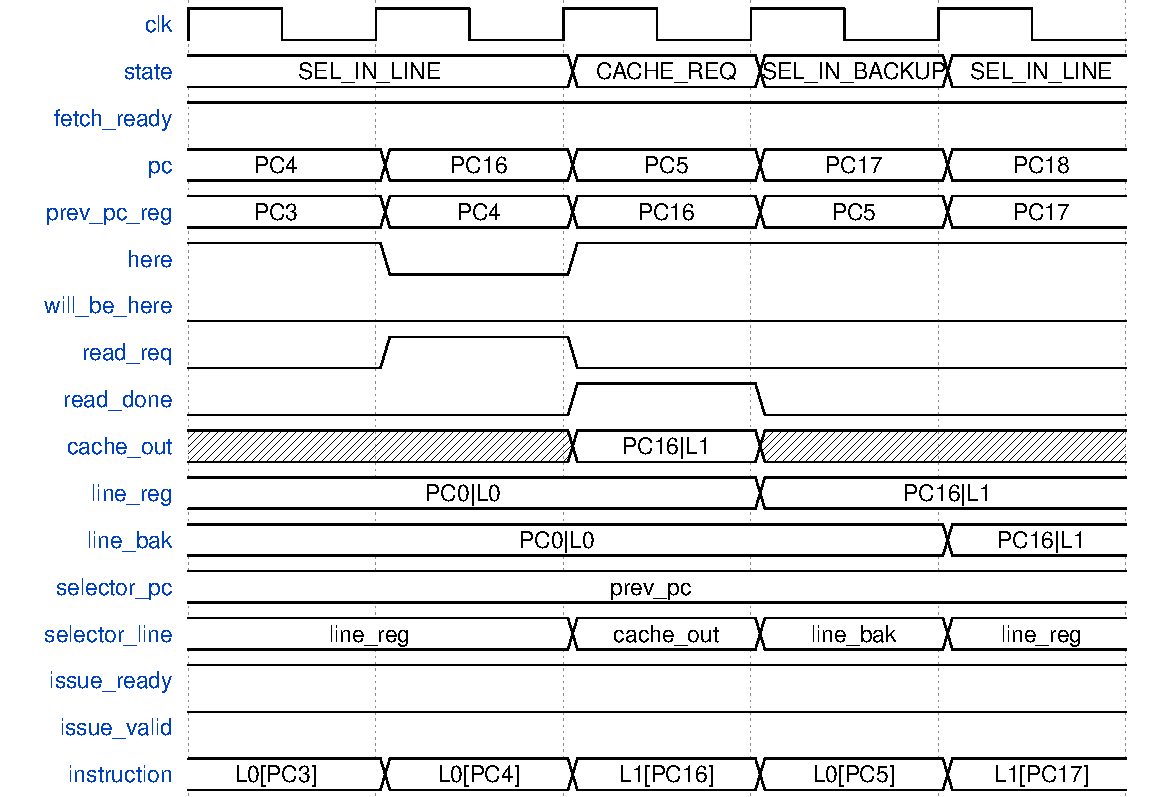
\includegraphics[width=\textwidth]{img/fetch09.pdf}
  \caption{Line backup register purpose}
  \label{fig:fetch09}
\end{figure}
The purpose of the line backup register is demonstrated in the timing of \cref{fig:fetch09}, when there is a jump back and forth between two cache lines: the \texttt{here} signal during the cache request makes the next instruction be selected from the backup register. Of course, as already mentioned, the limitation of this solution is that if the same jump were to happen just right after this scenario (e.g. if \texttt{PC5} arrived again instead of \texttt{PC18} at the last shown cycle) even the backup register would have been overwritten and so a new memory access would be needed anyway.

\begin{figure}[!ht]
  \centering
  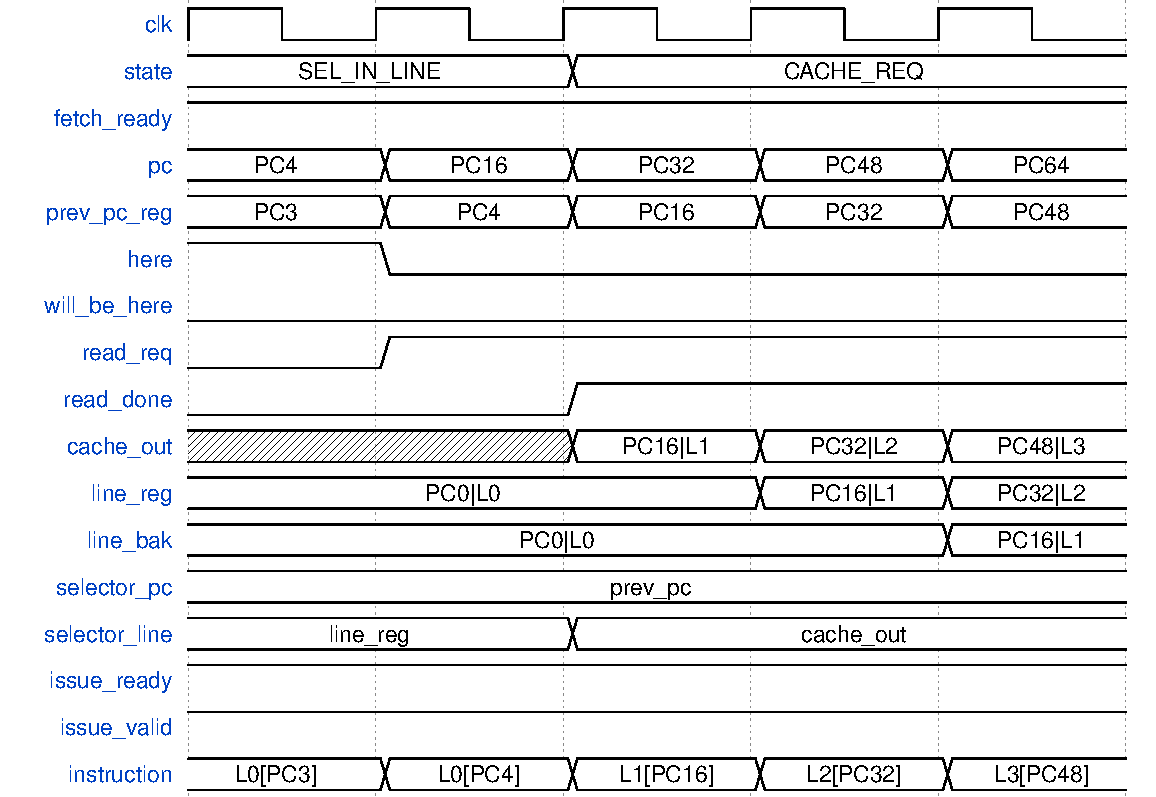
\includegraphics[width=\textwidth]{img/fetch07.pdf}
  \caption{Cache read pipeline}
  \label{fig:fetch07}
\end{figure}
\Cref{fig:fetch07} illustrates the ability to reach a throughput of one instruction per clock cycle in a pipeline fashion even while reading from the instruction cache, if the memory hits on every address. In this case instructions are always selected directly from the cache output.

\pagebreak
\begin{figure}[!ht]
  \centering
  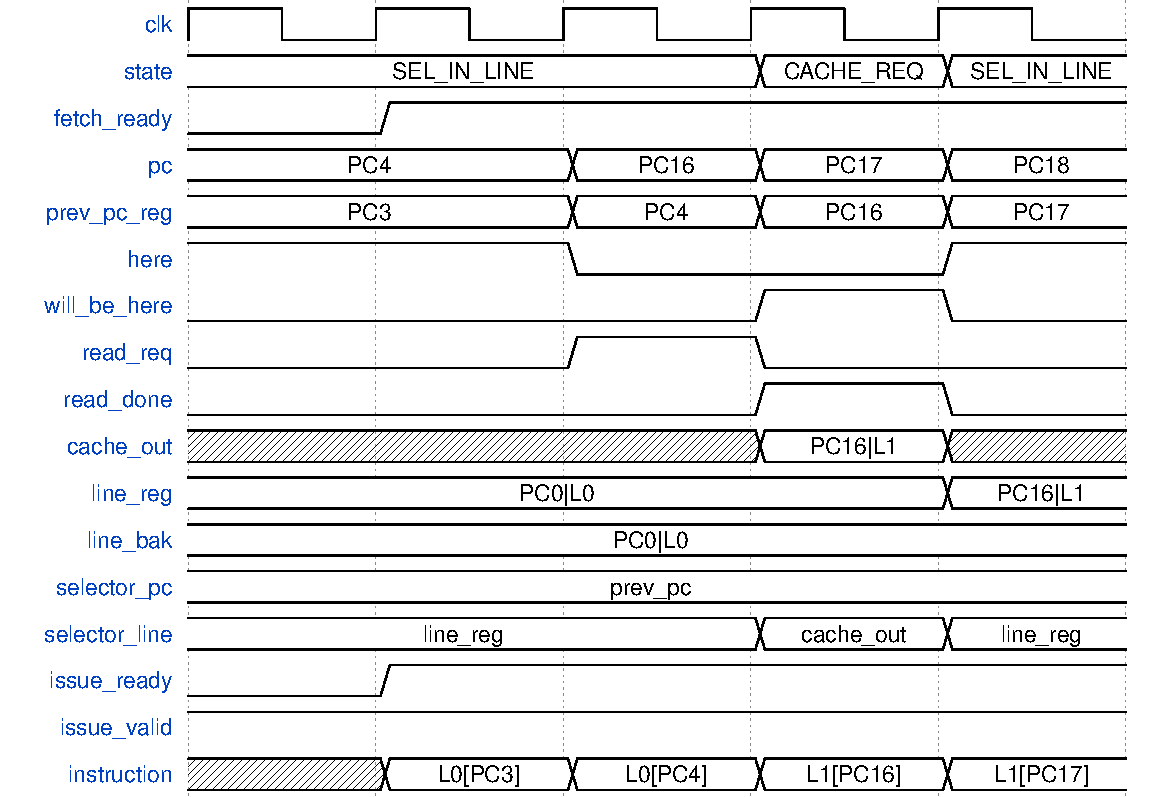
\includegraphics[scale=.65]{img/fetch03.pdf}
  \caption{Issue queue not ready during selection}
  \label{fig:fetch03}
\end{figure}
\begin{figure}[!ht]
  \centering
  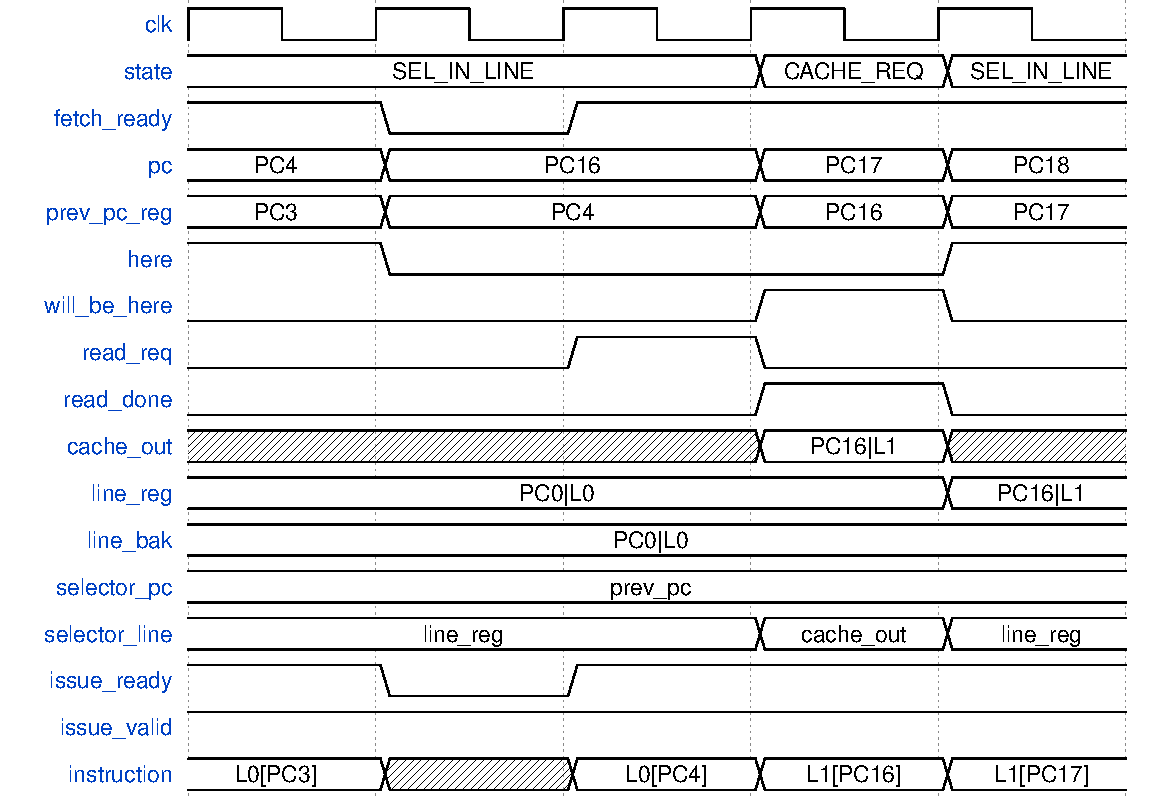
\includegraphics[scale=.65]{img/fetch04.pdf}
  \caption{Issue queue not ready during request}
  \label{fig:fetch04}
\end{figure}
\Cref{fig:fetch03,fig:fetch04} show the issue queue being not ready at two different instants. In \cref{fig:fetch03} the stall happens when the instruction is selected inside the line register and in this case no problem arises, as the fetch stage is simply stalled and no register changes until the issue queue becomes ready again. If the queue is busy when an address would require a cache read, as in \cref{fig:fetch04}, then the actual memory access is delayed until this stall is resolved. \todo{C'mon, solve this} In both cases, the \texttt{fetch\_ready} signal is deasserted to prevent the generation of new program counters.

\pagebreak
\begin{figure}[!ht]
  \centering
  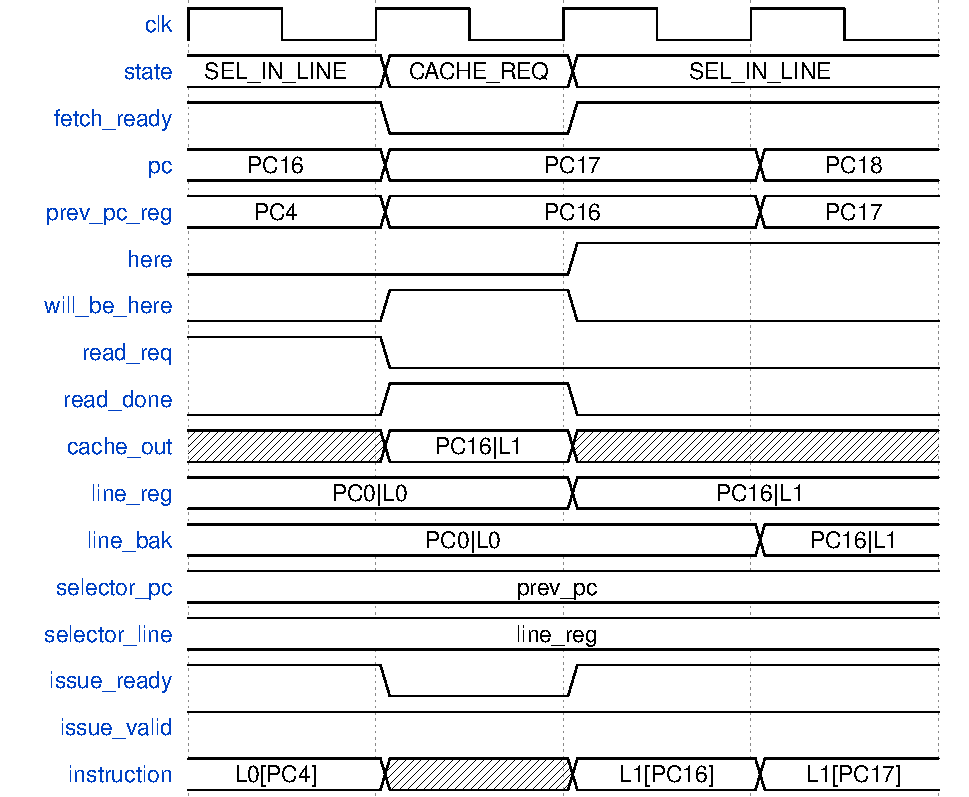
\includegraphics[width=.9\textwidth]{img/fetch05.pdf}
  \caption{Issue queue not ready when cache line arrives}
  \label{fig:fetch05}
\end{figure}
\Cref{fig:fetch05} shows the case for which the issue queue is not ready when the cache hits and outputs a new line and the current address points to an instruction in that line (\texttt{will\_be\_here} asserted). In this case, there is a stall when no new \ac{PC} is generated and during which the newly read line is saved into the line register, so that when the issue queue becomes ready again the instruction will be selected from the register and not from the cache output.

\begin{figure}[!ht]
  \centering
  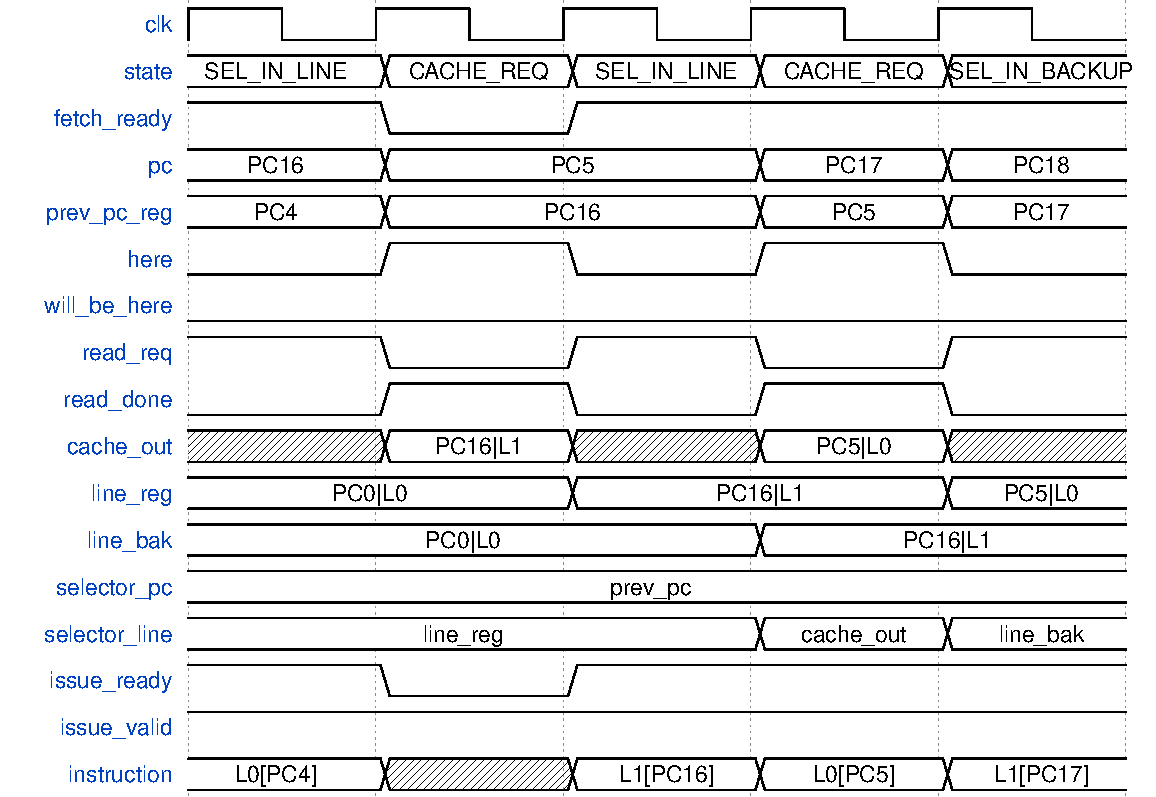
\includegraphics[scale=.65]{img/fetch08.pdf}
  \caption{Issue queue not ready and causing loss of backup}
  \label{fig:fetch08}
\end{figure}
The situation shown in \cref{fig:fetch08} is similar to the previous one, but this time the issue queue is not ready when the output is a new line and the current instruction refers to a line previously saved. In this case not even the line backup register can manage it, because as soon as the fetch resume, it is updated with the content of the line register, that is the last cache line read. Thus, for the old line a new memory access is required.

\begin{figure}[!ht]
  \centering
  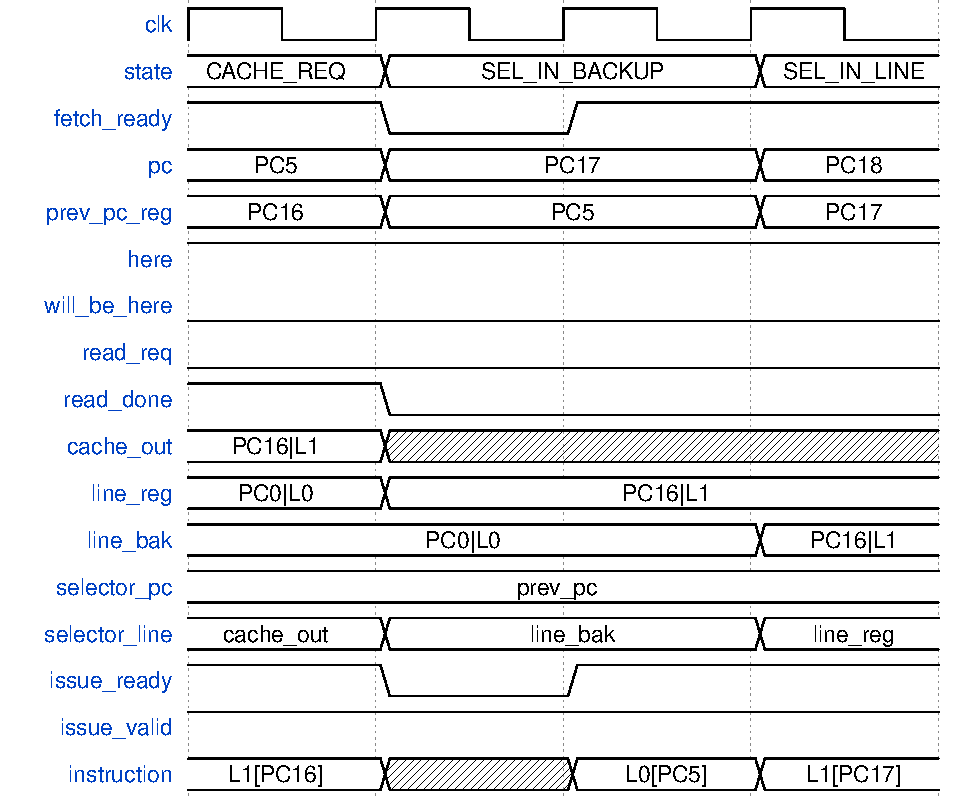
\includegraphics[scale=.65]{img/fetch10.pdf}
  \caption{Issue queue not ready during backup}
  \label{fig:fetch10}
\end{figure}
Finally, \cref{fig:fetch10} shows the last timing under analysis, that is the situation in which the issue is not ready when the instruction has to be selected inside the backup register. In similar manner to \cref{fig:fetch03}, here the stall does not cause any issues and the fetch resumes exactly as before when the queue turns ready again.

\section{\acf{BPU}}
As seen in \cref{fig:frontend}, the \ac{BPU} resides in the fetch stage and works in parallel with the \ac{IFU} on each address coming from the \ac{PC} gen stage. This unit, as shown in the high level scheme of \cref{fig:bpu-idea}, is composed of two main blocks:
\begin{figure}[hbt]
  \centering
  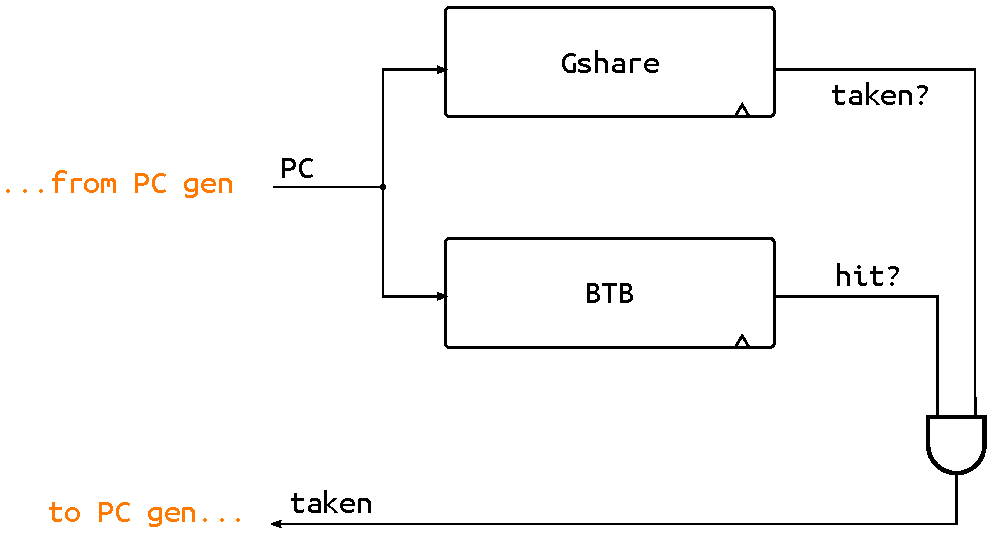
\includegraphics[width=.9\textwidth]{img/bpu-idea.pdf}
  \caption{\acs{BPU} general idea}
  \label{fig:bpu-idea}
\end{figure}
\begin{itemize}
  \item The \textbf{gshare} is the actual branch predictor and is a variation of the two-level predictor described in \cref{sec:twolevelbp} featuring a table of 2-bit counters and a global history register, of which a detailed explanation is provided in \cref{sec:gshare}. Being a branch predictor, its output is the predicted direction of the branch. Note that it outputs a prediction on every address, even those who potentially do not correspond to branch instructions. That is where the second block comes into play.
  \item The \textbf{\acf{BTB}}, described in \cref{sec:btb}, is a small cache that contains the target address of taken branches only. This provides the significant advantage of being able to fetch the instruction after the taken branch with no additional delay, leading to zero overhead branches if the target is correct.
\end{itemize}
A branch is predicted taken by the \ac{BPU} if and only if the gshare predictor supposes the branch is taken and the \ac{BTB} contains an entry with a valid target for that specific \ac{PC}.

\subsection{Top-level block diagram}
\begin{figure}[hbt]
  \centering
  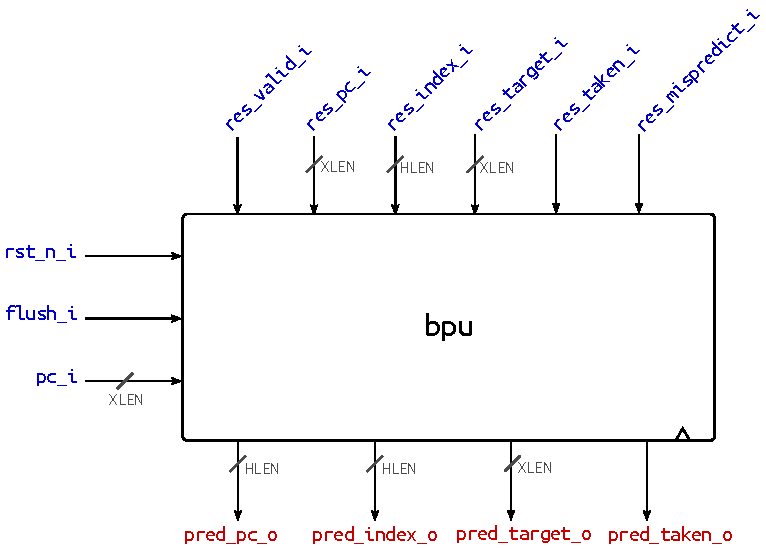
\includegraphics[width=.9\textwidth]{img/bpu-top.pdf}
  \caption{\acs{BPU} module ports}
  \label{fig:bpu-top}
\end{figure}
\Cref{fig:bpu-top} shows the module interface of the \ac{BPU}. Apart from reset and flush signals, used respectively at startup and in case an exception requires the internal data structures to be flushed, the module outputs a prediction based on the current address, composed by a single bit indicating if the branch is supposed to be taken or not, the predicted target and also the branch address, which is later needed to update the predictor structures.

The inputs containing the \texttt{res} prefix, for resolution, are the just mentioned branch \ac{PC} to which the resolution refers, the actual target, the actual branch direction, a bit indicating if there was a misprediction and a valid bit to signal that the present one is a valid branch resolution coming from the execution stage.

\begin{table}[hbt]
  \centering
  \makebox[\textwidth][c]{
    \begin{tabular}{llll}
      \toprule
      \textbf{Prediction}         & \textbf{Resolution}         & \textbf{Target}             & \textbf{Action} \\
      \midrule
      Taken                       & Taken                       & Correct                     & Increment 2-bit counter \\
      \midrule
      \multirow{3}{*}{Taken}      & \multirow{3}{*}{Taken}      & \multirow{3}{*}{Incorrect}  & Increment 2-bit counter \\
                                  &                             &                             & Update BTB entry \\
                                  &                             &                             & Flush pipeline and restart from correct target \\
      \midrule
      \multirow{3}{*}{Taken}      & \multirow{3}{*}{Not taken}  & \multirow{3}{*}{--}         & Decrement 2-bit counter \\
                                  &                             &                             & Remove BTB entry \\
                                  &                             &                             & Flush pipeline and restart from branch \ac{PC}+4 \\
      \midrule
      Not taken                   & Not taken                   & --                          & Decrement 2-bit counter \\
      \midrule
      \multirow{3}{*}{Not taken}  & \multirow{3}{*}{Taken}      & \multirow{3}{*}{--}         & Increment 2-bit counter \\
                                  &                             &                             & Add BTB entry \\
                                  &                             &                             & Flush pipeline and restart from correct target \\
      \bottomrule          
    \end{tabular}
  }
  \caption{Predictor update actions}
  \label{tab:bpupdate}
\end{table}
This information, in particular the two bits about the actual branch direction and the misprediction, is used to update the data structures and take further action as listed in \cref{tab:bpupdate}. In case of correct prediction, it is only needed to update the 2-bit counters inside the gshare predictor according to the branch direction. A misprediction, on the other hand, requires different actions to be taken depending on which event caused it. If the branch was correctly predicted taken, but the target in the \ac{BTB} was incorrect, then the \ac{BTB} entry must be updated with the correct one. If, instead, the branch was mispredicted taken, the target buffer entry is deleted in order to prevent a potential further misprediction, in the case when the 2-bit counter was in the \emph{strongly taken} state. Finally, if the branch was mispredicted not taken, then the corresponding target is added to the \ac{BTB}. This time, if the 2-bit counter was in the \emph{strongly not taken} state, the second misprediction cannot be prevented and the same entry will be written once again in the \ac{BTB}.

In all the misprediction cases, the fetch and execution stages must be flushed and the next \ac{PC} must be set to the next sequential address after the branch \ac{PC} if the branch was actually not taken, or to the correct target if the branch was actually taken. Note that this flush operation is different from the flush caused by an exception because, obviously, it does not reset the branch predictor structures, which are only updated with the correct branch result.

\begin{figure}[p]
  \centering
  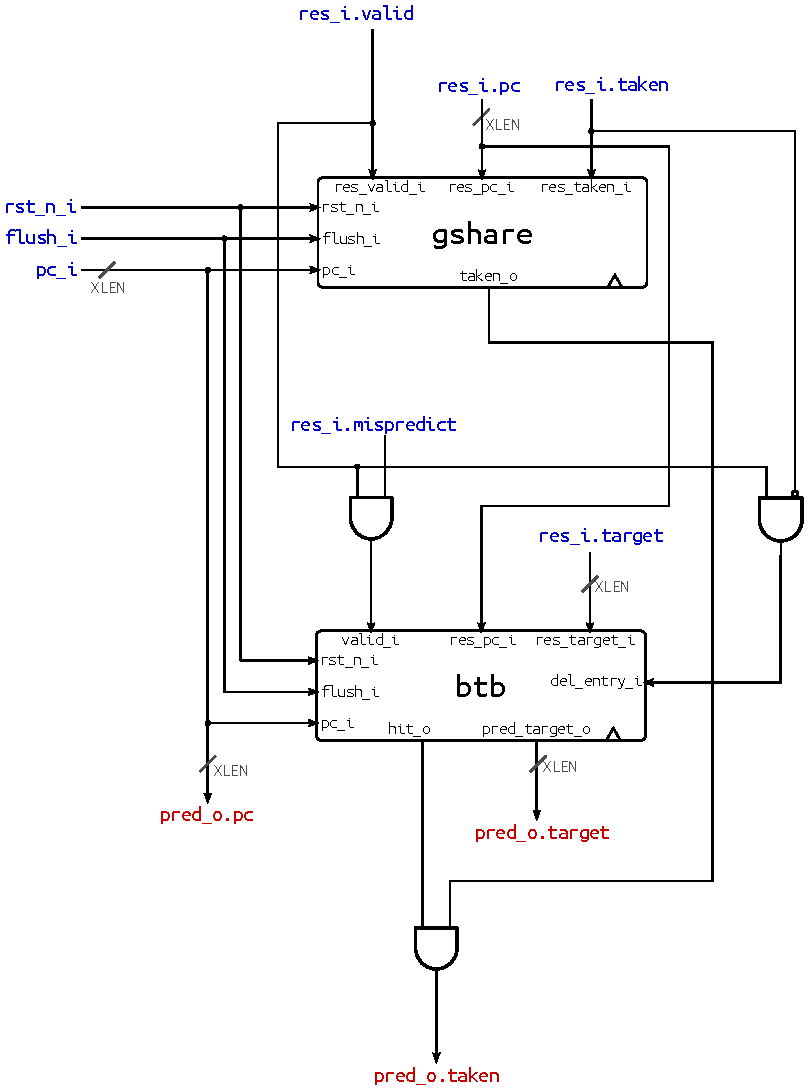
\includegraphics[width=\textwidth]{img/bpu.pdf}
  \caption{\acs{BPU} block diagram}
  \label{fig:bpu}
\end{figure}
\Cref{fig:bpu} shows the internal organization of the \ac{BPU} which is simply composed of the gshare and \ac{BTB} blocks, along with the AND gate of \cref{fig:bpu-idea} and a couple of other gates to decide the correct update action based on the results, as in \cref{tab:bpupdate}.

\pagebreak
\subsection{Gshare branch predictor}\label{sec:gshare}
\begin{figure}[hbt]
  \centering
  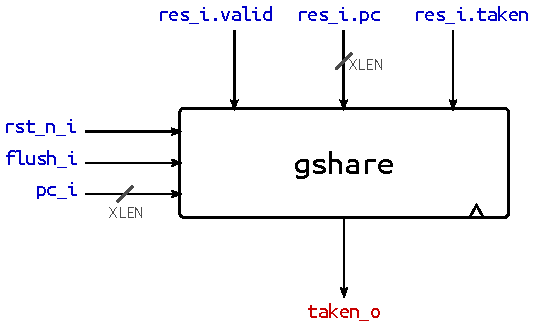
\includegraphics{img/gshare-top.pdf}
  \caption{Gshare module ports}
  \label{fig:gshare-top}
\end{figure}
The idea of the gshare predictor, whose interface is shown in \cref{fig:gshare-top}, was first proposed by Scott McFarling in a 1993 paper \cite{mcfarling93} and consists in a variation of the two-level predictor that combines global information from the global branch history and local information of the current branch address by hashing them with the exclusive OR of the history register and the $N$ least significant bits of the \ac{PC}, where $N$ is the history length. The author noted that this hashed index contains more information useful to identify the current branch than each of the \ac{PC} and global history alone and the experimental results confirmed this thesis, by outperforming all previous variations of the two-level predictor.

\begin{figure}[hbt]
  \centering
  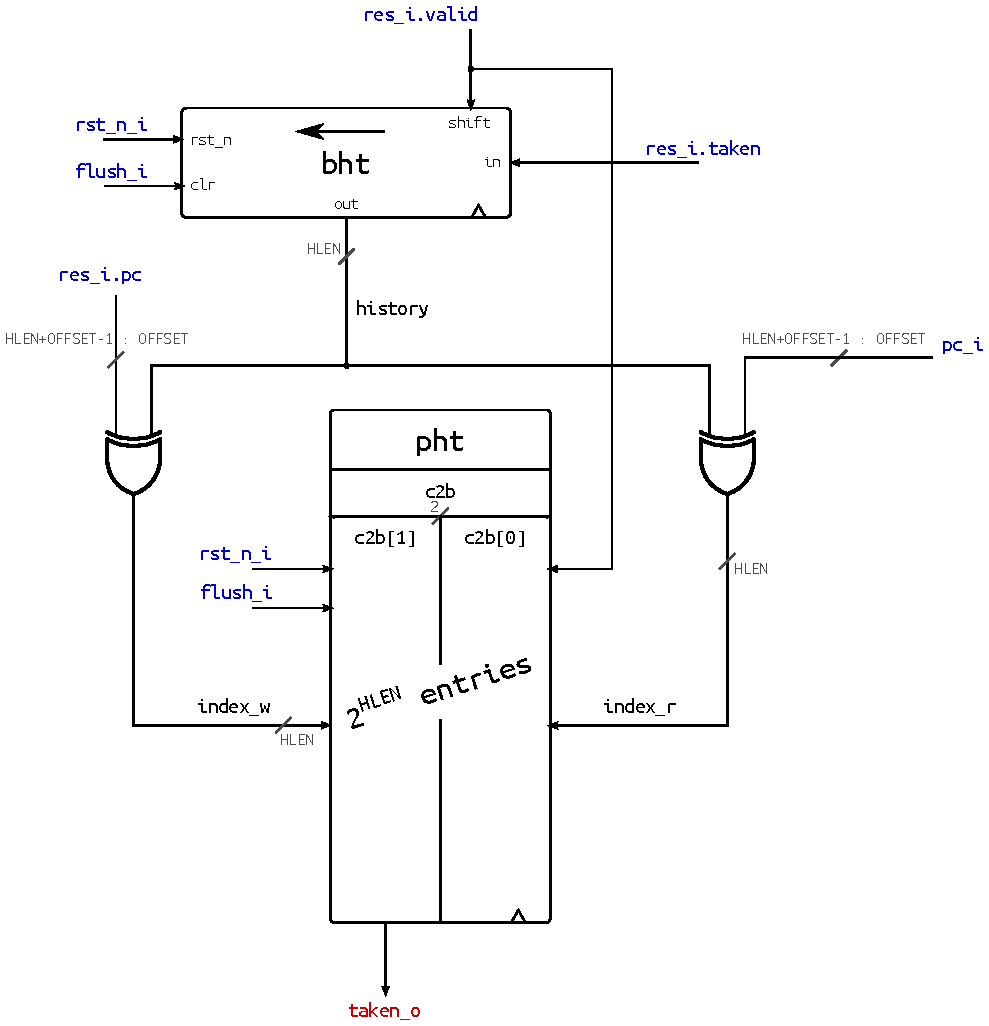
\includegraphics[width=\textwidth]{img/gshare.pdf}
  \caption{Gshare branch predictor}
  \label{fig:gshare}
\end{figure}
The structure of this predictor is shown in \cref{fig:gshare} and is composed of a \ac{BHT} composed of a single shift register where branch resolutions are left shifted in and a \ac{PHT} that contains an array of 2-bit counters, organized as a register file, so providing synchronous write and asynchronous read. This table is indexed by the XOR of the history and the current \ac{PC}\footnote{Actually, the 2 LSBs of the \ac{PC} are excluded as are always zero for 32-bit instruction.} in order to read the prediction for the current branch, which comes from the most significant bit of the 2-bit counter.

\begin{figure}[hbt]
  \vspace{2cm}
  \centering
  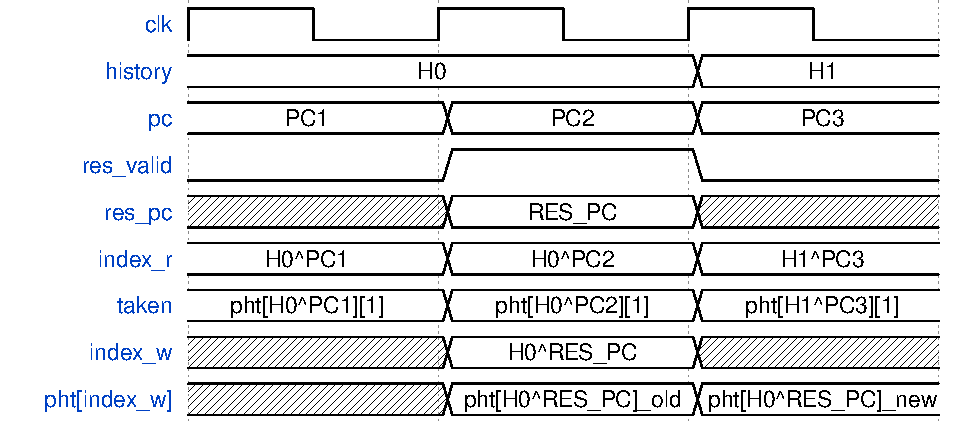
\includegraphics[width=\textwidth]{img/gshare01.pdf}
  \caption{Update timing diagram}
  \label{fig:gshare01}
\end{figure}
To update the \ac{PHT} when a branch is resolved the correct 2-bit counter has to be selected using the same index as the one used for the prediction. As an architectural choice, branches in LEN5 are resolved in-order during the execution stages, so that in the time span between the prediction and the resolution of a branch, no other resolution is generated and as such the branch history remains unchanged. This means that the write index used to select the 2-bit counter to be updated can be derived using the resolved branch address and the same current value of the history register. This poses no timing issues, as demonstrated by \cref{fig:gshare01}, because the history register is shifted only after the clock edge when the \texttt{res\_valid} signal is active, so at that edge the register still stores the unshifted value and the write operation on the \ac{PHT} occurs at the correct address.

If branches were resolved \ooo, on the other hand, to restore the correct address to the \ac{PHT} the index at the moment of the prediction would need to be passed along in the pipeline to return at the moment of the resolution. Resolving branches in-order, on the other hand, not only allows a significant size reduction of data structures like the issue queue and the branch reservation stations by not storing the prediction index, but also simplifies a great deal the instruction commit stage.

The initial version of the design also accounted for a column of valid bits in the \ac{PHT} to indicate if the prediction coming from each 2-bit counter is valid (i.e.\ if that 2-bit counter has already been used at least once). This is useful to prevent taken misprediction if the 2-bit counters are initialized in the weakly or strongly taken state. However, if the counters are instead initialized in a not taken state, then the first time they are accessed the prediction will always be ``not taken'' just as if the valid bit was included, so this bit becomes redundant and only wastes area. After a more thorough analysis, presented in \cref{sec:gshare_bench}, it was decided to remove the valid bits from the \ac{PHT}.

\pagebreak
\subsection{\acf{BTB}}\label{sec:btb}
\begin{figure}[hbt]
  \centering
  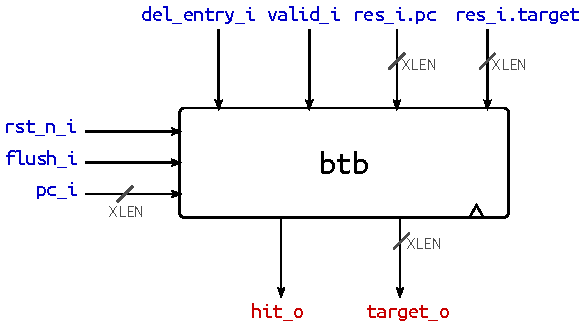
\includegraphics{img/btb-top.pdf}
  \caption{\acs{BTB} module ports}
  \label{fig:btb-top}
\end{figure}
The purpose of the \ac{BTB} (interface in \cref{fig:btb-top}) is to provide the target of a predicted taken branch in order to eliminate the delay of the computation of the destination address in the later execution stages and allow the fetch to proceed immediately from the new address. The idea of a \ac{BTB} was first introduced in \cite{lee84} and was since optimized and employed in a great number of processor designs.

\begin{figure}[hbt]
  \vspace{2cm}
  \centering
  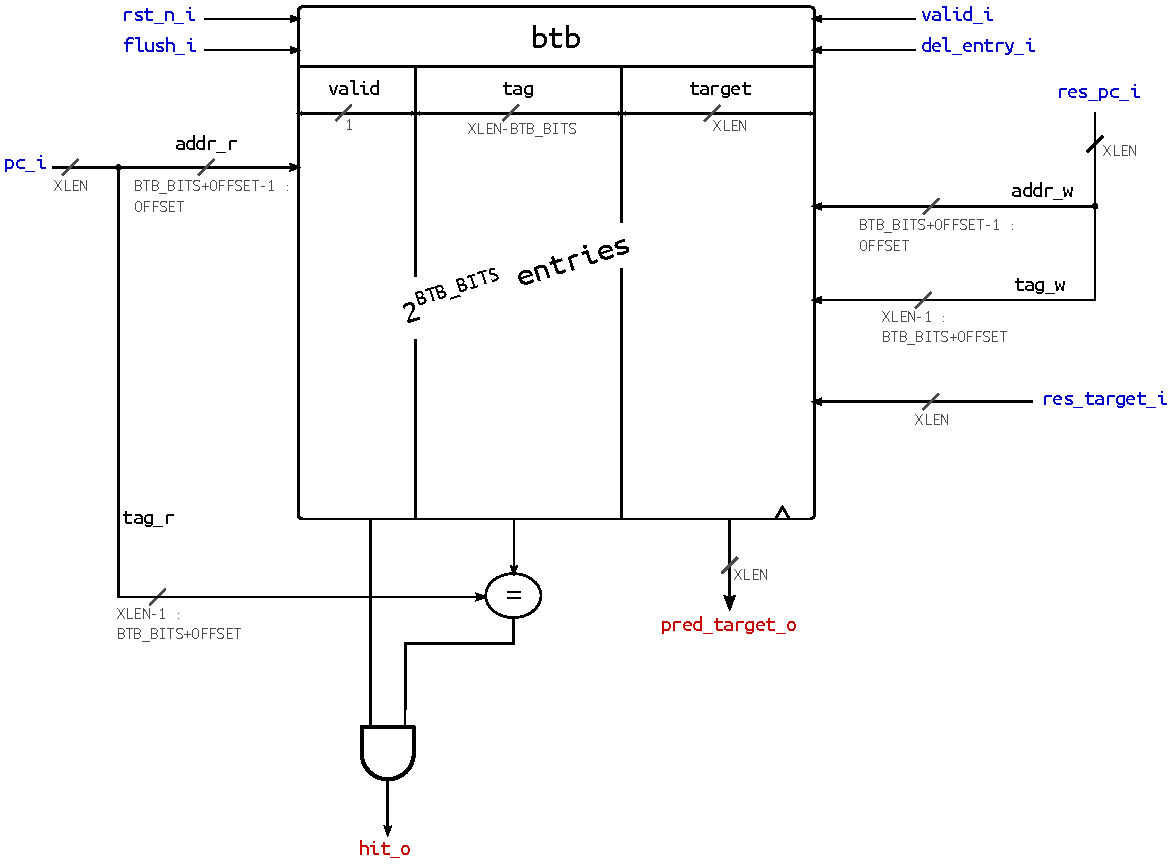
\includegraphics[width=\textwidth]{img/btb.pdf}
  \caption{\acs{BTB} diagram}
  \label{fig:btb}
\end{figure}
Its structure shown in \cref{fig:btb} is basically that of a direct mapped cache with $2^{\texttt{BTB\_BITS}}$ entries addressed using the the \texttt{BTB\_BITS} least significant bits of the \ac{PC}, as always excluding the offset, where each of them contains the following fields:
\begin{itemize}
  \item \textbf{Valid}: 1-bit field indicating if the selected entry is valid, that is if it has been previously written with the correct target of a resolved branch.
  \item \textbf{Tag}: this field contains the remaining bits of the branch \ac{PC} not used to address the \ac{BTB}. The final evaluation on the branch address is a hit only if for the selected location the valid bit is set and the stored tag corresponds to the upper part of the \ac{PC}. This is done in order to eliminate the aliasing phenomenon, for which multiple addresses could point to the same \ac{BTB} entry and thus produce incorrect results for the target. 
  \item \textbf{Target}: the actual destination address of the branch. The 2 LSBs are not stored as are they are useless for 32-bit instructions, but can save a significant amount of area if the \ac{BTB} contains many entries.
\end{itemize}
When the \texttt{del\_entry} signal is asserted all three fields of the addressed entry are reset to zero.

\pagebreak
The \ac{BTB} is perhaps one of the blocks that can organized and optimized in the most number of ways, starting from the mapping of the cache to the information stored. Some variants of the design store the actual target instruction instead of the address to allow for some advanced techniques such as branch folding \cite{perleberg93}. Being LEN5 an exploratory experiment on processor design, the choice has been made to keep the organization simple and so implement the \ac{BTB} as a direct mapped cache described as a register file.

For this reason, the same principles presented in \cref{sec:gshare} apply here, namely that the \ac{BTB} allows synchronous write and asynchronous read that in turn imply that a prediction and an update can be completed during the same cycle.
% HERE
\pagebreak
\section{Branch unit}
A unit that was not talked about until now and that is not shown in \cref{fig:frontend} because it resides in the backend is the branch unit, which is an execution unit responsible of determining the actual outcome of branch instructions. Its main tasks are the logic comparison between operand values in order to determine if the branch is taken or not and the sum of the base branch address and its immediate field to discover the target.

\begin{figure}[hbt]
  \centering
  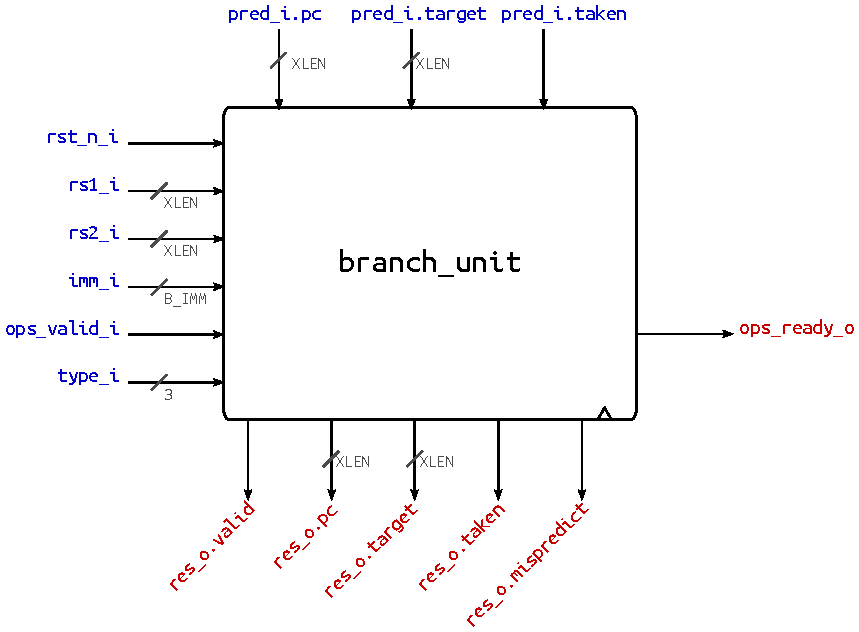
\includegraphics[width=.9\textwidth]{img/branch_unit-top.pdf}
  \caption{Branch unit module ports}
  \label{fig:branch_unit-top}
\end{figure}
\Cref{fig:branch_unit-top} shows the interface ports of this unit. It receives the register operands \texttt{rs1} and \texttt{rs2}, the immediate field \texttt{imm} the branch type, encoded on three bits, and the prediction information from the corresponding reservation station, to and from which it communicates via the handshake signals \texttt{ops\_valid} and \texttt{ops\_ready} as usual.

Its outputs are the information on the branch resolution, which is passed forward to the commit stage and back to the frontend to update the \ac{BPU} and potentially stall in case of misprediction.

\subsection{Datapath}
\begin{figure}[hbt]
  \centering
  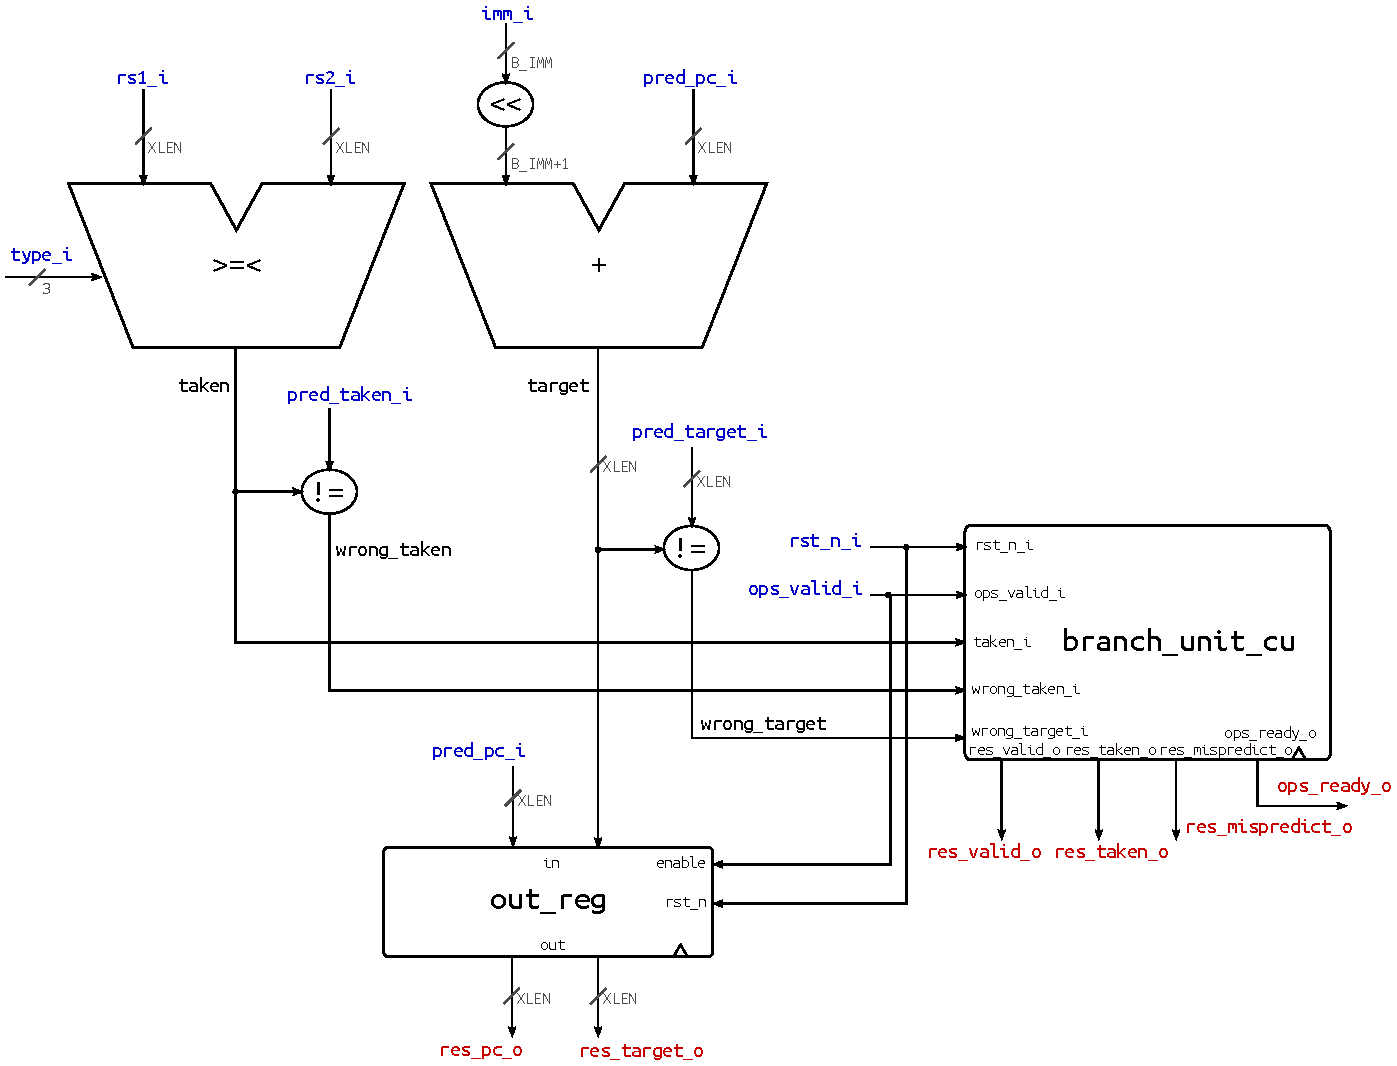
\includegraphics[width=\textwidth]{img/branch_unit.pdf}
  \caption{Branch unit datapath}
  \label{fig:branch_unit}
\end{figure}
The datapath of the branch unit is shown in \cref{fig:branch_unit} and is composed of two ALUs, which are actually a separate logic unit and an adder, operating in parallel on the comparison and the target computation, which is performed, as per \riscv specifications, by adding the base address with the immediate left shifted. The output of both units is compared with the predicted taken and target respectively and the results are passed to the control unit.

There are six types of branches in the \riscv \ac{ISA}, namely:
\begin{itemize}
  \item Branch if equal (\texttt{BEQ})
  \item Branch if not equal (\texttt{BNE})
  \item Branch if less than (\texttt{BLT})
  \item Branch if greater than or equal (\texttt{BGE})
  \item Branch if less than, unsigned (\texttt{BLTU})
  \item Branch if greater than or equal (\texttt{BGEU})
\end{itemize}

At the following clock cycle after the ALUs have obtained the results, the control unit outputs the correct prediction information and the branch \ac{PC} and right target are written to the output register.

\subsection{Control unit}
\begin{figure}[hbt]
  \centering
  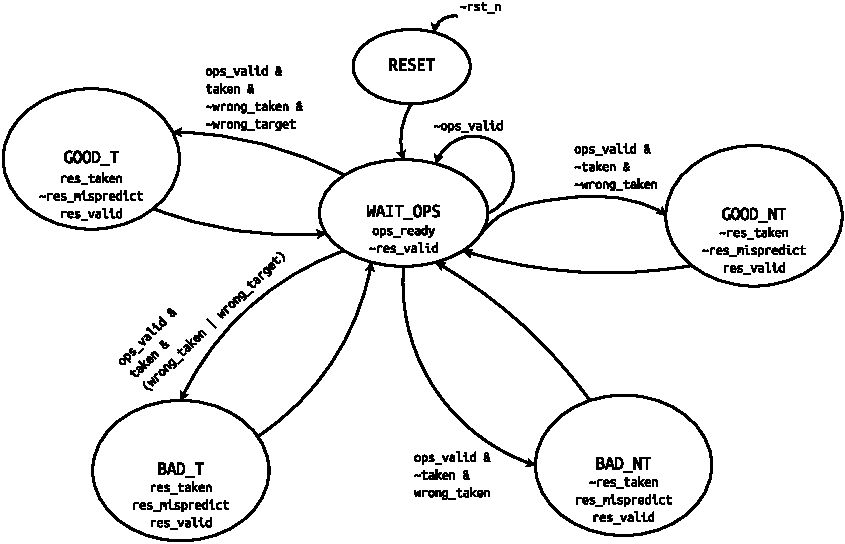
\includegraphics[width=\textwidth]{img/branch_unit_fsm.pdf}
  \caption{Branch unit control unit}
  \label{fig:branch_unit_fsm}
\end{figure}
The control unit of this module is a Moore machine that after reset starts waiting for valid operands from the reservation station in the \texttt{WAIT\_OPS} state. When they arrive, in the same clock cycle the datapath performs the required computation, so that according to the value of the control signals, the \acs{FSM} can move to one of the states named \texttt{{GOOD,BAD}\_{T,NT}}, based on whether there was misprediction and whether the branch was actually taken or not. In these states, the correct output signals are driven and then the state machine moves back to the waiting loop.
\todo{Aggiungere timing dopo modifica}
